\documentclass[letterpaper,12pt,twoside,]{pinp}

%% Some pieces required from the pandoc template
\providecommand{\tightlist}{%
  \setlength{\itemsep}{0pt}\setlength{\parskip}{0pt}}

% Use the lineno option to display guide line numbers if required.
% Note that the use of elements such as single-column equations
% may affect the guide line number alignment.

\usepackage[T1]{fontenc}
\usepackage[utf8]{inputenc}

% pinp change: the geometry package layout settings need to be set here, not in pinp.cls
\geometry{layoutsize={0.95588\paperwidth,0.98864\paperheight},%
  layouthoffset=0.02206\paperwidth, layoutvoffset=0.00568\paperheight}

\definecolor{pinpblue}{HTML}{185FAF}  % imagecolorpicker on blue for new R logo
\definecolor{pnasbluetext}{RGB}{101,0,0} %



\title{An Introduction to ggplot2: the grammar of graphics}

\author[a]{Martin Frigaard}

  \affil[a]{CSU, Chico}

\setcounter{secnumdepth}{0}

% Please give the surname of the lead author for the running footer
\leadauthor{}

% Keywords are not mandatory, but authors are strongly encouraged to provide them. If provided, please include two to five keywords, separated by the pipe symbol, e.g:
 \keywords{  ggplot2 |  RStudio  }  

\begin{abstract}
\texttt{ggplot2} is part of the \texttt{tidyverse}, which is a
collection of opinionated packages from RStudio that
\href{https://www.tidyverse.org/packages/}{`\emph{you're likely to use
in everyday data analyses.}'}.
\end{abstract}

\dates{This version was compiled on \today} 


% initially we use doi so keep for backwards compatibility
% new name is doi_footer
\doifooter{\url{https://mjfrigaard.github.io/csuc-data-journalism/}}


\begin{document}

% Optional adjustment to line up main text (after abstract) of first page with line numbers, when using both lineno and twocolumn options.
% You should only change this length when you've finalised the article contents.
\verticaladjustment{-2pt}

\maketitle
\thispagestyle{firststyle}
\ifthenelse{\boolean{shortarticle}}{\ifthenelse{\boolean{singlecolumn}}{\abscontentformatted}{\abscontent}}{}

% If your first paragraph (i.e. with the \dropcap) contains a list environment (quote, quotation, theorem, definition, enumerate, itemize...), the line after the list may have some extra indentation. If this is the case, add \parshape=0 to the end of the list environment.


\hypertarget{objectives}{%
\section{Objectives}\label{objectives}}

\begin{itemize}
\item[$\square$]
  Explain why there is as Grammar of Graphics is and the problem it
  solves
\item[$\square$]
  Understand how the pipe makes code easier to write (and read)
\item[$\square$]
  Define the terms \texttt{geom} and \texttt{aesthetic}
\item[$\square$]
  Compare and contrast function calls with and without the pipe operator
\item[$\square$]
  Create a visualization using \texttt{ggplot2}'s quickplot function
  (\texttt{qplot()})
\item[$\square$]
  Build a graph one layer at a time using the \texttt{ggplot} template
\end{itemize}

\hypertarget{what-is-ggplot2}{%
\section{\texorpdfstring{What is
\texttt{ggplot2}?}{What is ggplot2?}}\label{what-is-ggplot2}}

The \texttt{ggplot2} package is an implementation of the
\href{https://amzn.to/2MRRCAB}{``Grammar of Graphics''} by Leland
Wilkinson. This text outlines a foundation for understanding the
components of just about every graph or figure we've encountered (and
some we haven't). \texttt{ggplot2} extends these concepts into a
powerful grammar for developing data visualizations in R.

\hypertarget{why-have-a-grammar-of-data-visualization}{%
\subsection{\texorpdfstring{\textbf{\emph{Why have a `grammar' of data
visualization?}}}{Why have a `grammar' of data visualization?}}\label{why-have-a-grammar-of-data-visualization}}

\href{https://en.wikipedia.org/wiki/Wilhelm_von_Humboldt}{Wilhelm von
Humboldt} has described a language as a system for ``\emph{making
infinite use of finite means.}'' Grammar is the set of rules we use to
generate and display comprehensible thought (to humans or computers).
Within the R language, \texttt{ggplot2} provides the grammar (or set of
rules) we can learn to develop a rich vocabulary for data
visualizations. Knowing how to use \texttt{ggplot2}'s grammar also gives
us an excellent mental model for thinking about individual graphical
elements.

\hypertarget{the-lingua-franca-for-graphical-elements}{%
\subsection{\texorpdfstring{\textbf{\emph{The lingua franca for
graphical
elements}}}{The lingua franca for graphical elements}}\label{the-lingua-franca-for-graphical-elements}}

We'll extend the definition of `grammar' above to include Steven
Pinker's description of language in
\href{https://www.amazon.com/Sense-Style-Thinking-Persons-Writing/dp/0143127799}{The
Sense of Style}, ``\emph{{[}language is{]} our species' solution to the
problem of getting complicated thoughts from one head into another}.''
In this sense, the \texttt{ggplot2} package gives us an ability to
communicate the \emph{complexities} of our data in the same way that
scientific jargon allows us to precisely and unambiguously define ideas.

\hypertarget{building-graphs-bit-by-bit}{%
\subsection{\texorpdfstring{\textbf{\emph{Building graphs,
bit-by-bit}}}{Building graphs, bit-by-bit}}\label{building-graphs-bit-by-bit}}

Lastly, \texttt{ggplot2} has an expansive vocabulary, so by learning a
finite list of \texttt{ggplot2} functions and their syntax will allow us
to build a seemingly unlimited number of visualizations.

\hypertarget{the-tidyverse-and-the-pipe}{%
\section{\texorpdfstring{The \texttt{tidyverse} and the pipe
(\texttt{\%\textgreater{}\%})}{The tidyverse and the pipe (\%\textgreater\%)}}\label{the-tidyverse-and-the-pipe}}

Load the \texttt{tidyverse} package by typing or copying and pasting the
code below.

\begin{Shaded}
\begin{Highlighting}[]
\FunctionTok{install.packages}\NormalTok{(}\StringTok{"tidyverse"}\NormalTok{)}
\FunctionTok{library}\NormalTok{(tidyverse)}
\end{Highlighting}
\end{Shaded}

A major reason for using the \texttt{tidyverse} is the pipe operator
from the \href{https://magrittr.tidyverse.org/}{\texttt{magrittr}
package}.

\hypertarget{the-pipe}{%
\subsection{\texorpdfstring{\textbf{\emph{the pipe
\texttt{\%\textgreater{}\%}}}}{the pipe \%\textgreater\%}}\label{the-pipe}}

The pipe (\texttt{\%\textgreater{}\%}) is what's referred to as
syntactic sugar (yes, that's
\href{https://en.wikipedia.org/wiki/Syntactic_sugar}{really a term})
because it's,

``\emph{syntax within a programming language that is designed to make
things easier to read or to express}''

\hypertarget{using-the-pipe}{%
\subsection{\texorpdfstring{\textbf{\emph{Using the pipe
\texttt{\%\textgreater{}\%}}}}{Using the pipe \%\textgreater\%}}\label{using-the-pipe}}

Writing R code using the pipe operator makes it easier to combine
function calls, and it's easier for to read. For example, consider a
single function call:

\begin{center}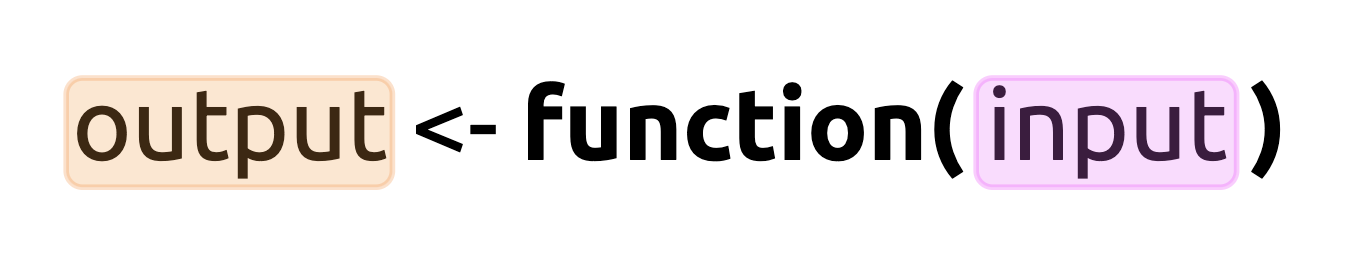
\includegraphics[width=4in,height=1in]{../img/pipe-args-01} \end{center}

The pipe allows us to write this as, ``take the \emph{input} and apply
this \emph{function()}''

\begin{center}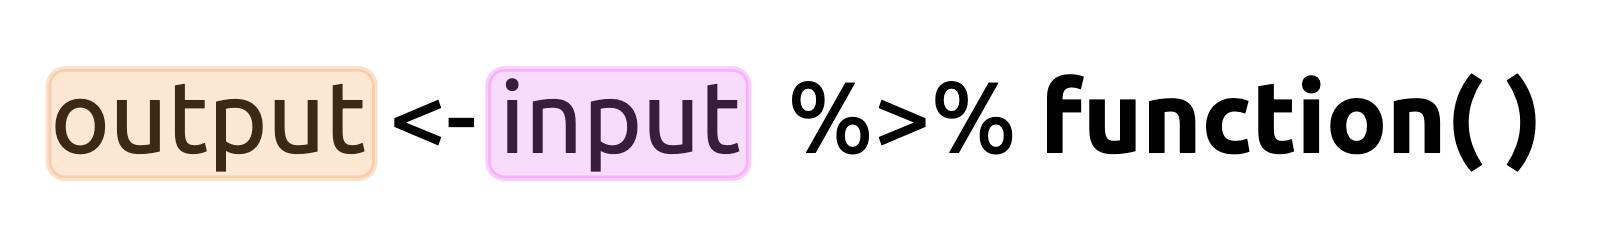
\includegraphics[width=5in,height=1in]{../img/pipe-args-02} \end{center}

Writing code this way might not seem like it's a big improvement in
clarity, but consider a more complicated series of function calls:

\begin{center}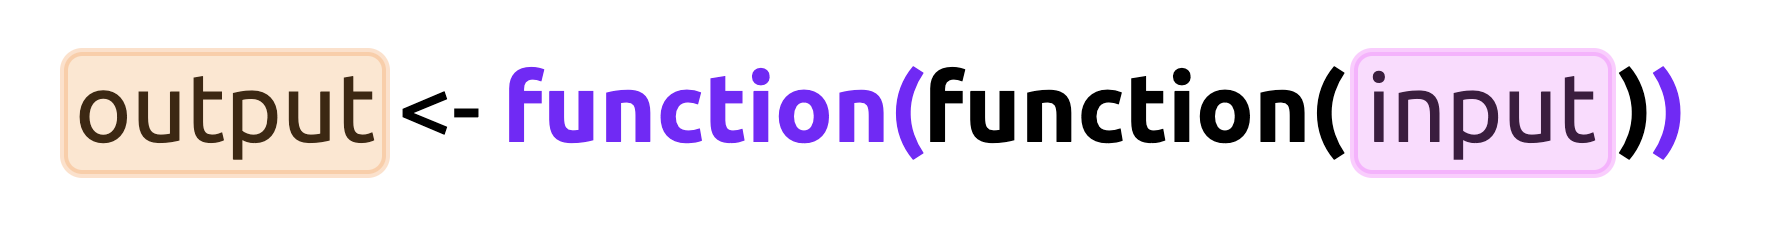
\includegraphics[width=5.7in,height=1in]{../img/pipe-args-03} \end{center}

If we want to apply a two functions, we have to write them so the output
from the first function is an input for the second function--which means
they have to written inside-out!

If we use the pipe operator, the code looks like this:

\begin{center}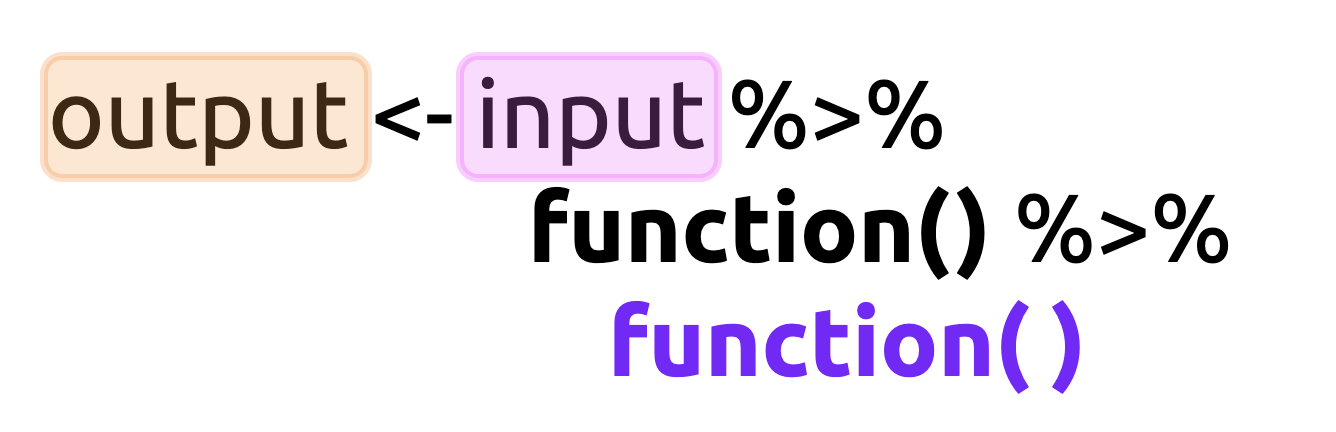
\includegraphics[width=4.2in,height=1.5in]{../img/pipe-args-04} \end{center}

Now we can take the \textbf{\texttt{input}}, apply the first
\textbf{\texttt{function()}}, then pass the output from the first
function to the second \textbf{\texttt{function()}} and store this in
the \textbf{\texttt{output}}.

\hypertarget{ggplot2-geoms-and-aesthetics}{%
\section{\texorpdfstring{ggplot2: \texttt{geoms} and
\texttt{aes}thetics}{ggplot2: geoms and aesthetics}}\label{ggplot2-geoms-and-aesthetics}}

A \emph{geom} (or geometric object) is the `thing' we see on a graph or
plot (this includes dots or points, lines, bars, etc.).

\emph{geoms} are combined with aesthetic mappings, which are properties
of the `thing' on the plot or graph (this includes things like color,
size, position, and shape).

So every graph or plot has a geom, and that geom will also have some
visual properties called aesthetics.

\hypertarget{starting-with-quick-plots}{%
\subsection{\texorpdfstring{\textbf{\emph{Starting with quick
plots}}}{Starting with quick plots}}\label{starting-with-quick-plots}}

We will start using \texttt{ggplot2} with the \texttt{qplot()} function.
\texttt{qplot()} is short for `quick plot', and it takes the following
arguments:

\begin{Shaded}
\begin{Highlighting}[]
\NormalTok{ggplot2}\SpecialCharTok{::}\FunctionTok{qplot}\NormalTok{(}\AttributeTok{data =}\NormalTok{ Data, }\CommentTok{\# assume dataset \textquotesingle{}Data\textquotesingle{}}
               \AttributeTok{x =}\NormalTok{ variable\_x, }\CommentTok{\# single column on the x}
               \AttributeTok{y =}\NormalTok{ variable\_y, }\CommentTok{\# single column on the y}
               \AttributeTok{geom =} \StringTok{"shape"}\NormalTok{) }\CommentTok{\# the \textquotesingle{}thing\textquotesingle{} on the graph}
\end{Highlighting}
\end{Shaded}

Assume the same dataset \texttt{Data}, and two variables
\texttt{variable\_x} and \texttt{variable\_y}. If we wanted to use the
pipe with the \texttt{ggplot2::qplot()} function, it would look like the
code below:

\begin{Shaded}
\begin{Highlighting}[]
\NormalTok{Data }\SpecialCharTok{\%\textgreater{}\%}\NormalTok{ ggplot2}\SpecialCharTok{::}\FunctionTok{qplot}\NormalTok{(}\AttributeTok{data =}\NormalTok{ ., }\AttributeTok{x =}\NormalTok{ variable\_x, }\AttributeTok{y =}\NormalTok{ variable\_y, }\AttributeTok{geom =} \StringTok{"shape"}\NormalTok{)}
\end{Highlighting}
\end{Shaded}

\hypertarget{using-the-dot-.}{%
\subsection{\texorpdfstring{\textbf{\emph{Using the dot
(\texttt{.})}}}{Using the dot (.)}}\label{using-the-dot-.}}

\href{https://magrittr.tidyverse.org/}{\texttt{magrittr} package} has
some additional tricks that are worth knowing. For example, in the code
above, you may have noticed the \texttt{data\ =\ .} argument.

\begin{Shaded}
\begin{Highlighting}[]
\NormalTok{Data }\SpecialCharTok{\%\textgreater{}\%} 
\NormalTok{  ggplot2}\SpecialCharTok{::}\FunctionTok{qplot}\NormalTok{(}\AttributeTok{data =}\NormalTok{ ., }
                 \AttributeTok{x =}\NormalTok{ variable\_x, }
                 \AttributeTok{y =}\NormalTok{ variable\_y,}
                 \AttributeTok{geom =} \StringTok{"shape"}\NormalTok{)}
\end{Highlighting}
\end{Shaded}

The period (\texttt{.}) here is a product of the pipe syntax. We use the
\texttt{.} argument because of where the \texttt{data\ =} argument sits
inside the \texttt{qplot()} function. See the \texttt{args()} by using
\texttt{args(qplot)}

\begin{Shaded}
\begin{Highlighting}[]
\FunctionTok{args}\NormalTok{(qplot)}
\end{Highlighting}
\end{Shaded}

\begin{Shaded}
\begin{Highlighting}[]
\ControlFlowTok{function}\NormalTok{(x, y, ..., data, }
        \CommentTok{\# all other optional arguments}
        \AttributeTok{facets =} \ConstantTok{NULL}\NormalTok{, }
        \AttributeTok{margins =} \ConstantTok{FALSE}\NormalTok{, }
        \AttributeTok{geom =} \StringTok{"auto"}\NormalTok{, }
        \AttributeTok{xlim =} \FunctionTok{c}\NormalTok{(}\ConstantTok{NA}\NormalTok{, }\ConstantTok{NA}\NormalTok{), }
        \AttributeTok{ylim =} \FunctionTok{c}\NormalTok{(}\ConstantTok{NA}\NormalTok{, }\ConstantTok{NA}\NormalTok{), }
        \AttributeTok{log =} \StringTok{""}\NormalTok{, }
        \AttributeTok{main =} \ConstantTok{NULL}\NormalTok{, }
        \AttributeTok{xlab =} \ConstantTok{NULL}\NormalTok{, }
        \AttributeTok{ylab =} \ConstantTok{NULL}\NormalTok{, }
        \AttributeTok{asp =} \ConstantTok{NA}\NormalTok{, }
        \AttributeTok{stat =} \ConstantTok{NULL}\NormalTok{, }
        \AttributeTok{position =} \ConstantTok{NULL}\NormalTok{) }
\end{Highlighting}
\end{Shaded}

We can see the \texttt{data} argument comes \emph{after} the \texttt{x},
\texttt{y}, and any other variable arguments \texttt{...}. That means we
need to tell the pipe we want the \texttt{Data} to be in the named
\texttt{data\ =} argument, so we use \texttt{data\ =\ .}

So by using the pipe, we can rewrite this function,

\begin{Shaded}
\begin{Highlighting}[]
\ControlFlowTok{function}\NormalTok{(y, }\AttributeTok{named\_argument =}\NormalTok{ x)}
\end{Highlighting}
\end{Shaded}

to this:

\begin{Shaded}
\begin{Highlighting}[]
\NormalTok{x }\SpecialCharTok{\%\textgreater{}\%} \ControlFlowTok{function}\NormalTok{(y, }\AttributeTok{named\_argument =}\NormalTok{ .)}
\end{Highlighting}
\end{Shaded}

By placing the \texttt{data\ =\ .} on the right-hand side of the pipe
operator (\texttt{\%\textgreater{}\%}) in the \texttt{named\_argument}
position, we're telling R to read this statement as, ``\emph{the object
to the left of the \texttt{\%\textgreater{}\%} belongs in the
\texttt{data} argument.}''

See the figure below:

\begin{center}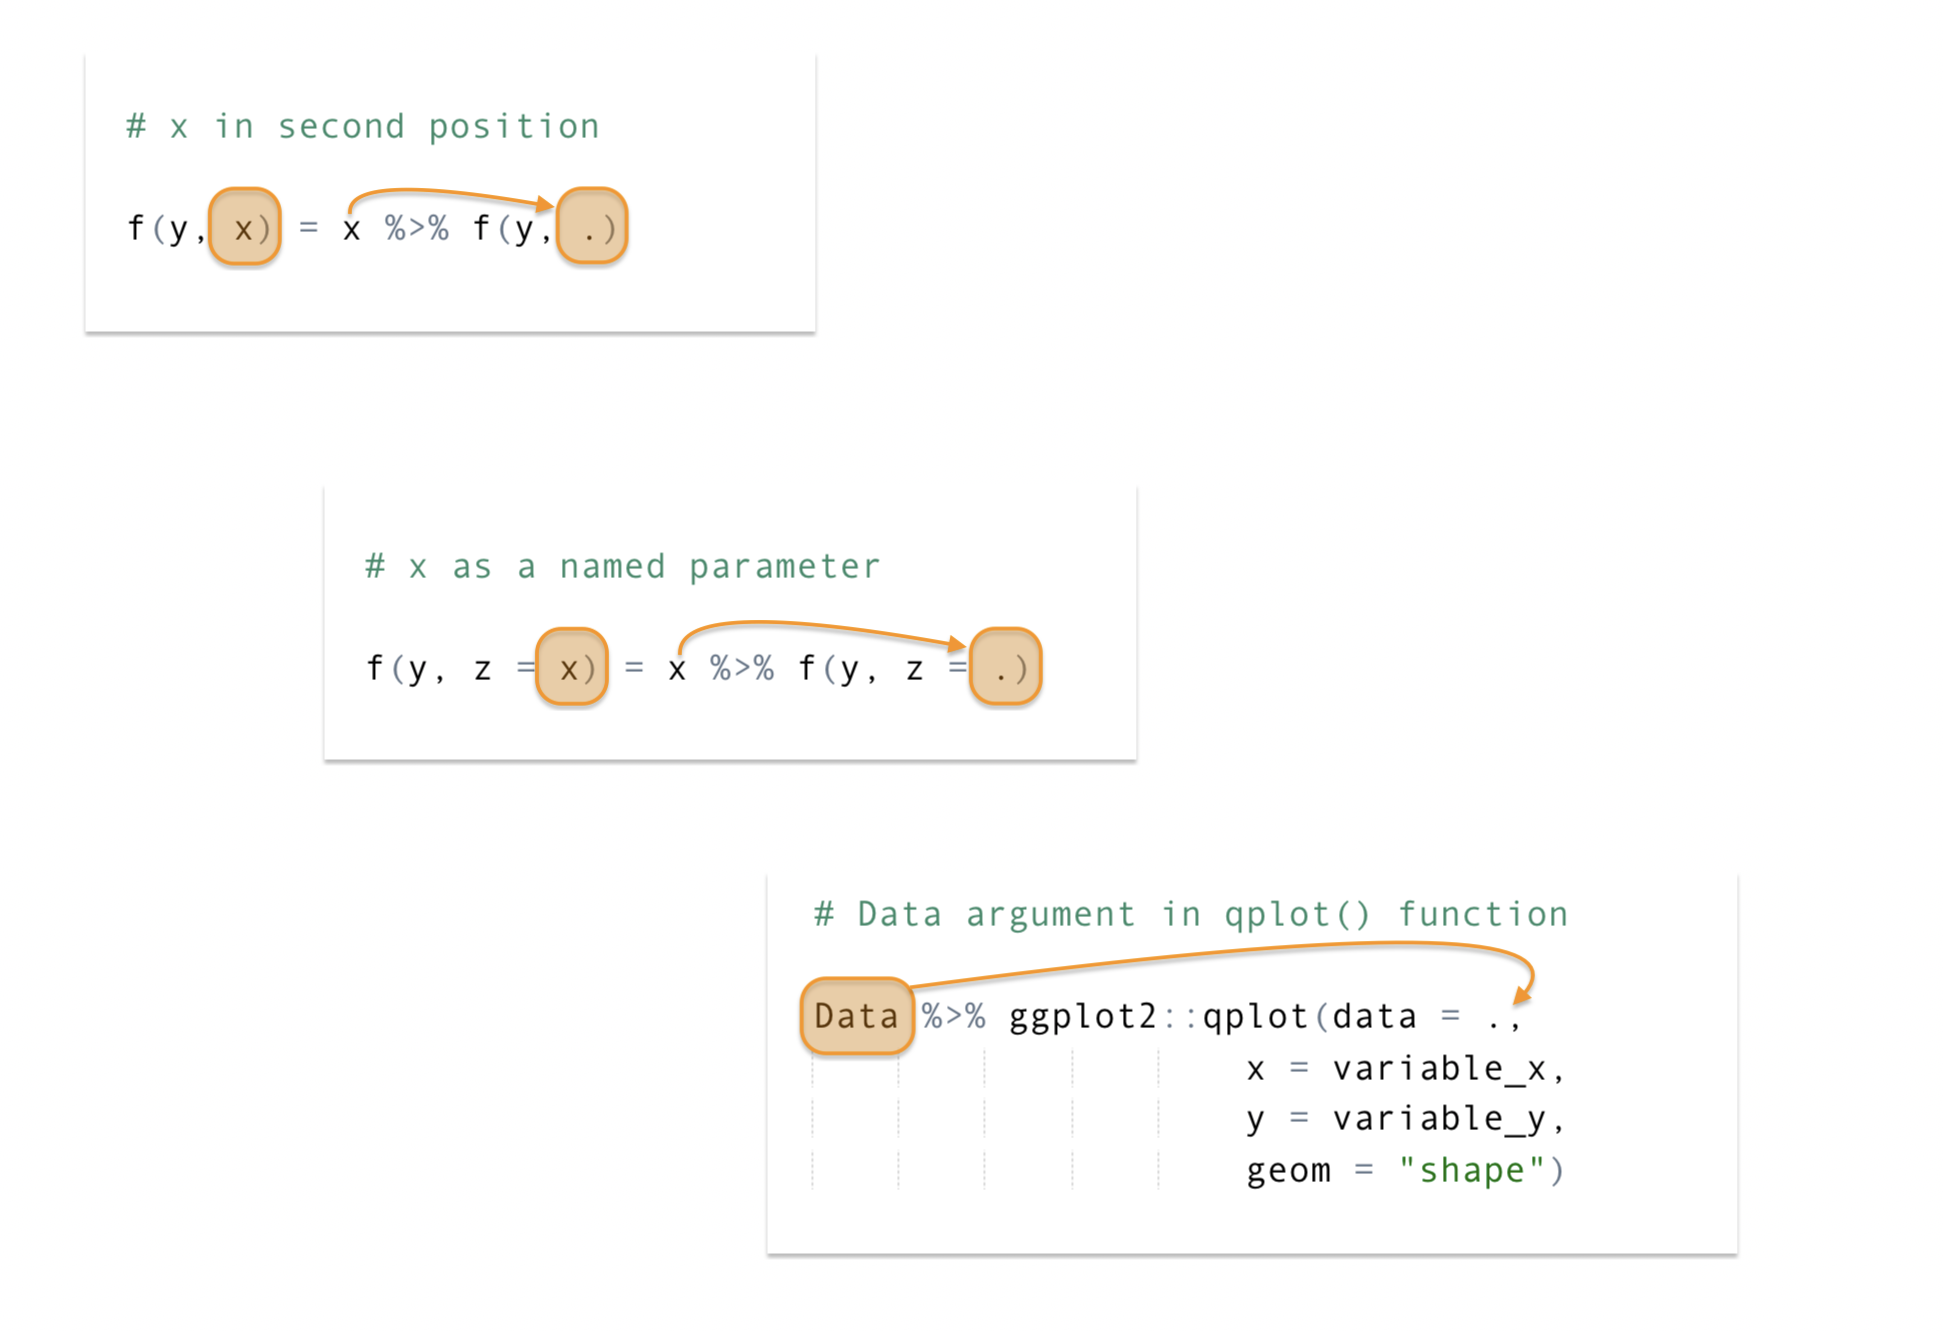
\includegraphics[width=6in,height=3in]{../img/pipe-data-args} \end{center}

We can demonstrate this in the code section below:

\begin{itemize}
\tightlist
\item
  First we create a \texttt{diamonds} dataset from the \texttt{ggplot2}
  package,
\item
  Then we `pipe' the data to \texttt{qplot()}
\end{itemize}

\begin{Shaded}
\begin{Highlighting}[]
\CommentTok{\# data }
\NormalTok{diamonds }\OtherTok{\textless{}{-}}\NormalTok{ ggplot2}\SpecialCharTok{::}\NormalTok{diamonds}
\CommentTok{\# graph}
\NormalTok{diamonds }\SpecialCharTok{\%\textgreater{}\%} 
\NormalTok{  ggplot2}\SpecialCharTok{::}\FunctionTok{qplot}\NormalTok{(}\AttributeTok{data =}\NormalTok{ ., }
                 \AttributeTok{x =}\NormalTok{ carat, }\AttributeTok{y =}\NormalTok{ price, }
                 \AttributeTok{geom =} \StringTok{"point"}\NormalTok{)}
\end{Highlighting}
\end{Shaded}

\begin{center}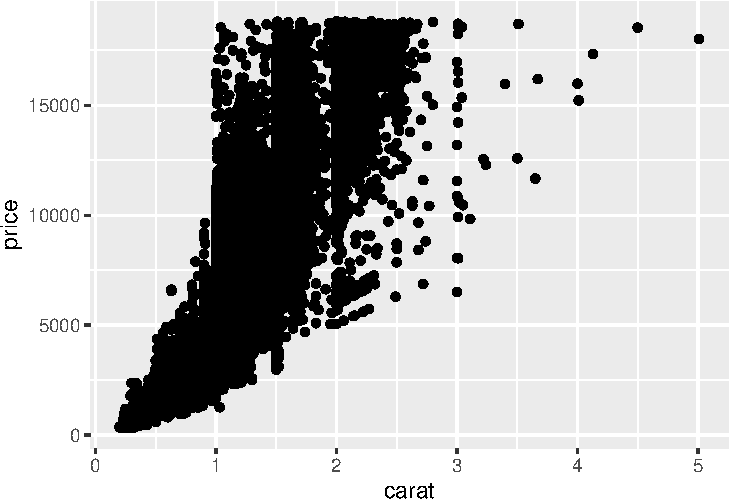
\includegraphics{03-intro-to-ggplot2_files/figure-latex/diamonds-qplot-1} \end{center}

\hypertarget{lets-get-some-data}{%
\section{Lets get some data!}\label{lets-get-some-data}}

We will be using \texttt{ggplot2} to explore data from the Economist's
Medium post titled,
\href{https://medium.economist.com/mistakes-weve-drawn-a-few-8cdd8a42d368}{``Mistakes,
we've drawn a few''}. These data are available for download as part of
the \href{https://github.com/rfordatascience/tidytuesday}{\#TidyTuesday}
project on Github.

The code section below will import the data into RStudio.

\begin{Shaded}
\begin{Highlighting}[]
\CommentTok{\# Balance }
\NormalTok{Balance }\OtherTok{\textless{}{-}}\NormalTok{ readr}\SpecialCharTok{::}\FunctionTok{read\_csv}\NormalTok{(}\StringTok{"https://bit.ly/3hRzrKS"}\NormalTok{)}
\CommentTok{\# Brexit }
\NormalTok{Brexit }\OtherTok{\textless{}{-}}\NormalTok{ readr}\SpecialCharTok{::}\FunctionTok{read\_csv}\NormalTok{(}\StringTok{"https://bit.ly/3s2wqMx"}\NormalTok{)}
\CommentTok{\# Corbyn }
\NormalTok{Corbyn }\OtherTok{\textless{}{-}}\NormalTok{ readr}\SpecialCharTok{::}\FunctionTok{read\_csv}\NormalTok{(}\StringTok{"https://bit.ly/35mgYRB"}\NormalTok{)}
\CommentTok{\# Pensions }
\NormalTok{Pensions }\OtherTok{\textless{}{-}}\NormalTok{ readr}\SpecialCharTok{::}\FunctionTok{read\_csv}\NormalTok{(}\StringTok{"https://bit.ly/2MNAvEp"}\NormalTok{)}
\end{Highlighting}
\end{Shaded}

The code below displays each dataset using three different functions:
\texttt{dplyr::glimpse()}, \texttt{utils::head()}, and
\texttt{utils::str()} (\emph{we learned about these functions in the
previous lessons and exercises})

\begin{Shaded}
\begin{Highlighting}[]
\NormalTok{Balance }\SpecialCharTok{\%\textgreater{}\%}\NormalTok{ dplyr}\SpecialCharTok{::}\FunctionTok{glimpse}\NormalTok{()}
\end{Highlighting}
\end{Shaded}

\begin{ShadedResult}
\begin{verbatim}
#  Rows: 266
#  Columns: 4
#  $ country      <chr> "Belgium", "Germany", "Estonia", "Ireland", "Greece", "Sp~
#  $ account_type <chr> "current", "current", "current", "current", "current", "c~
#  $ year         <dbl> 2009, 2009, 2009, 2009, 2009, 2009, 2009, 2009, 2009, 200~
#  $ value        <dbl> -3755.0, 141234.0, 360.0, -7912.1, -29323.0, -46191.0, -1~
\end{verbatim}
\end{ShadedResult}

\begin{Shaded}
\begin{Highlighting}[]
\NormalTok{Brexit }\SpecialCharTok{\%\textgreater{}\%}\NormalTok{ utils}\SpecialCharTok{::}\FunctionTok{head}\NormalTok{()}
\end{Highlighting}
\end{Shaded}

\begin{ShadedResult}
\begin{verbatim}
#  # A tibble: 6 x 3
#    date     percent_responding_right percent_responding_wrong
#    <chr>                       <dbl>                    <dbl>
#  1 2/8/16                         46                       42
#  2 9/8/16                         45                       44
#  3 17/08/16                       46                       43
#  4 23/08/16                       45                       43
#  5 31/08/16                       47                       44
#  6 14/09/16                       46                       43
\end{verbatim}
\end{ShadedResult}

\begin{Shaded}
\begin{Highlighting}[]
\NormalTok{Corbyn }\SpecialCharTok{\%\textgreater{}\%} \FunctionTok{tail}\NormalTok{()}
\end{Highlighting}
\end{Shaded}

\begin{ShadedResult}
\begin{verbatim}
#  # A tibble: 6 x 2
#    political_group avg_facebook_likes
#    <chr>                        <dbl>
#  1 Jeremy Corbyn                 5210
#  2 Labour Party                   845
#  3 Momentum                       229
#  4 Owen Smith                     127
#  5 Andy Burnham                   105
#  6 Saving Labour                   56
\end{verbatim}
\end{ShadedResult}

\begin{Shaded}
\begin{Highlighting}[]
\NormalTok{Pensions }\SpecialCharTok{\%\textgreater{}\%}\NormalTok{ utils}\SpecialCharTok{::}\FunctionTok{str}\NormalTok{()}
\end{Highlighting}
\end{Shaded}

\begin{ShadedResult}
\begin{verbatim}
#  spec_tbl_df [35 x 3] (S3: spec_tbl_df/tbl_df/tbl/data.frame)
#   $ country              : chr [1:35] "Australia" "Austria" "Belgium" "Brazil" ...
#   $ pop_65_percent       : num [1:35] 15.04 18.76 18.22 7.84 16.14 ...
#   $ gov_spend_percent_gdp: num [1:35] 5.2 13.86 10.36 12 4.31 ...
#   - attr(*, "spec")=
#    .. cols(
#    ..   country = col_character(),
#    ..   pop_65_percent = col_double(),
#    ..   gov_spend_percent_gdp = col_double()
#    .. )
#   - attr(*, "problems")=<externalptr>
\end{verbatim}
\end{ShadedResult}

We've provided some additional information on each datasets below:

\begin{itemize}
\item
  \texttt{Balance} is a dataset with countries, the country budget
  balance/current-account balance, the year, and the value in billions
  of euros.
\item
  \texttt{Brexit} is a dataset of Brexit poll opinions (with dates).
\item
  \texttt{Corbyn} is a dataset of average Facebook likes and political
  leaders/groups.
\item
  \texttt{Pensions} is a dataset of countries, percent of the country's
  population 65 years old or over, and the percent of government
  spending on pensions as a percent of GDP.
\end{itemize}

\hypertarget{variable-types}{%
\subsection{\texorpdfstring{\textbf{\emph{Variable
types}}}{Variable types}}\label{variable-types}}

Before we look at how variables relate to each other, we should get an
idea of how each variable looks independently, or it's
\href{https://en.wikipedia.org/wiki/List_of_probability_distributions}{distribution.}.

How we visualize a variable's distribution depends on whether it's
\textbf{continuous}, \textbf{categorical}, or \textbf{binary}.

\textbf{Continuous} variables mean they can be any value including
\texttt{0}--and are typically thought of as raw measurements (i.e.,
human body weight, speed, time in seconds, etc.). Continuous variables
also can have decimal values that make sense.

\textbf{Categorical} variables count discrete items or events, such as
Facebook `like's or the number of page views. Categorical variables are
different from continuous variables because they have a fixed set of
possible values (i.e., you can't have 1/2 a Facebook 'like').

A particular case of a categorical variable is a \textbf{binary}
variable, which only has two possible values (\texttt{0} or \texttt{1},
\texttt{alive} or \texttt{dead}, \texttt{yes} or \texttt{no}, etc.).

\hypertarget{visualize-a-single-variable-histograms}{%
\section{Visualize a single variable:
histograms}\label{visualize-a-single-variable-histograms}}

We will view the distribution of the \texttt{avg\_facebook\_likes} from
the \texttt{Corbyn} dataset using \texttt{ggplot2::qplot()}.

\begin{Shaded}
\begin{Highlighting}[]
\NormalTok{Corbyn }\SpecialCharTok{\%\textgreater{}\%} 
\NormalTok{    ggplot2}\SpecialCharTok{::}\FunctionTok{qplot}\NormalTok{(}\AttributeTok{x =}\NormalTok{ avg\_facebook\_likes, }\AttributeTok{data =}\NormalTok{ .) }
\end{Highlighting}
\end{Shaded}

\begin{center}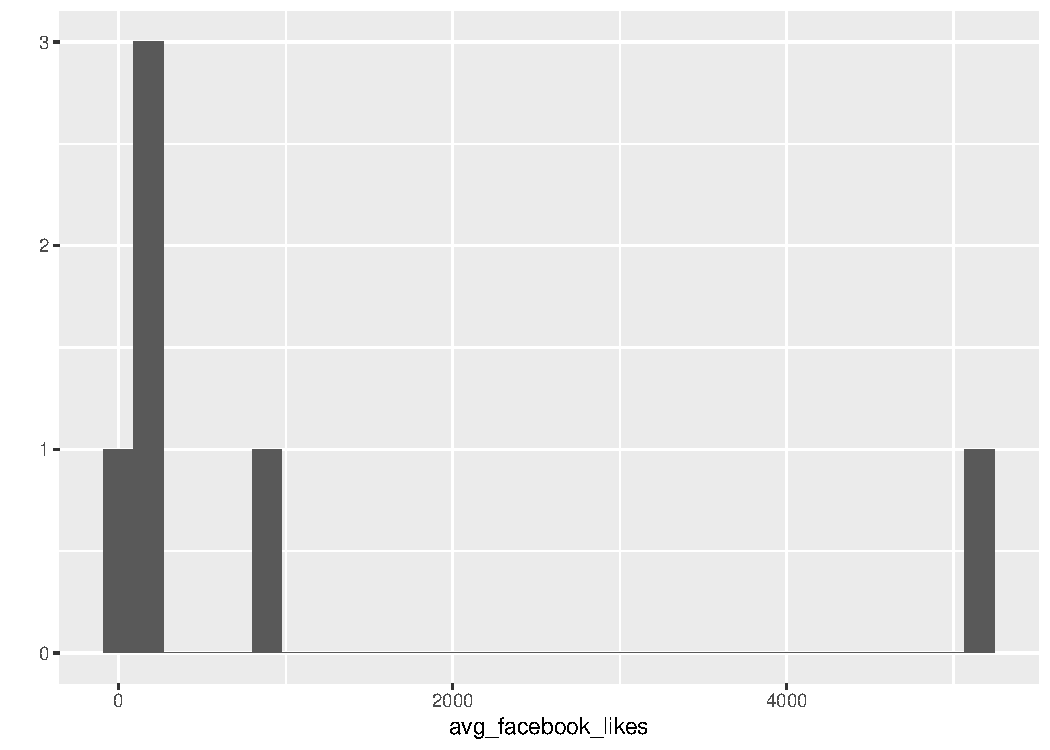
\includegraphics{03-intro-to-ggplot2_files/figure-latex/Corbyn-avg_facebook_likes-1} \end{center}

\emph{What is this graph telling us?}

Well, we can print the entire \texttt{Corbyn} dataset to the console to
view it (it's not very big).

We can see the data printed to the screen has the
\texttt{avg\_facebook\_likes} variable sorted descending, with the
highest number on top (\texttt{5210}), and the lowest number on the
bottom (\texttt{56}).

When we give the \texttt{qplot()} function a single numerical variable,
it assumes we want a
\href{https://ggplot2.tidyverse.org/reference/geom_histogram.html}{histogram}.

The histogram displays the \texttt{avg\_facebook\_likes} variable by
splitting up the \texttt{x} axis into \texttt{bins}, then plotting the
count for each number of observations in each bin on the \texttt{y}
axis.

\begin{center}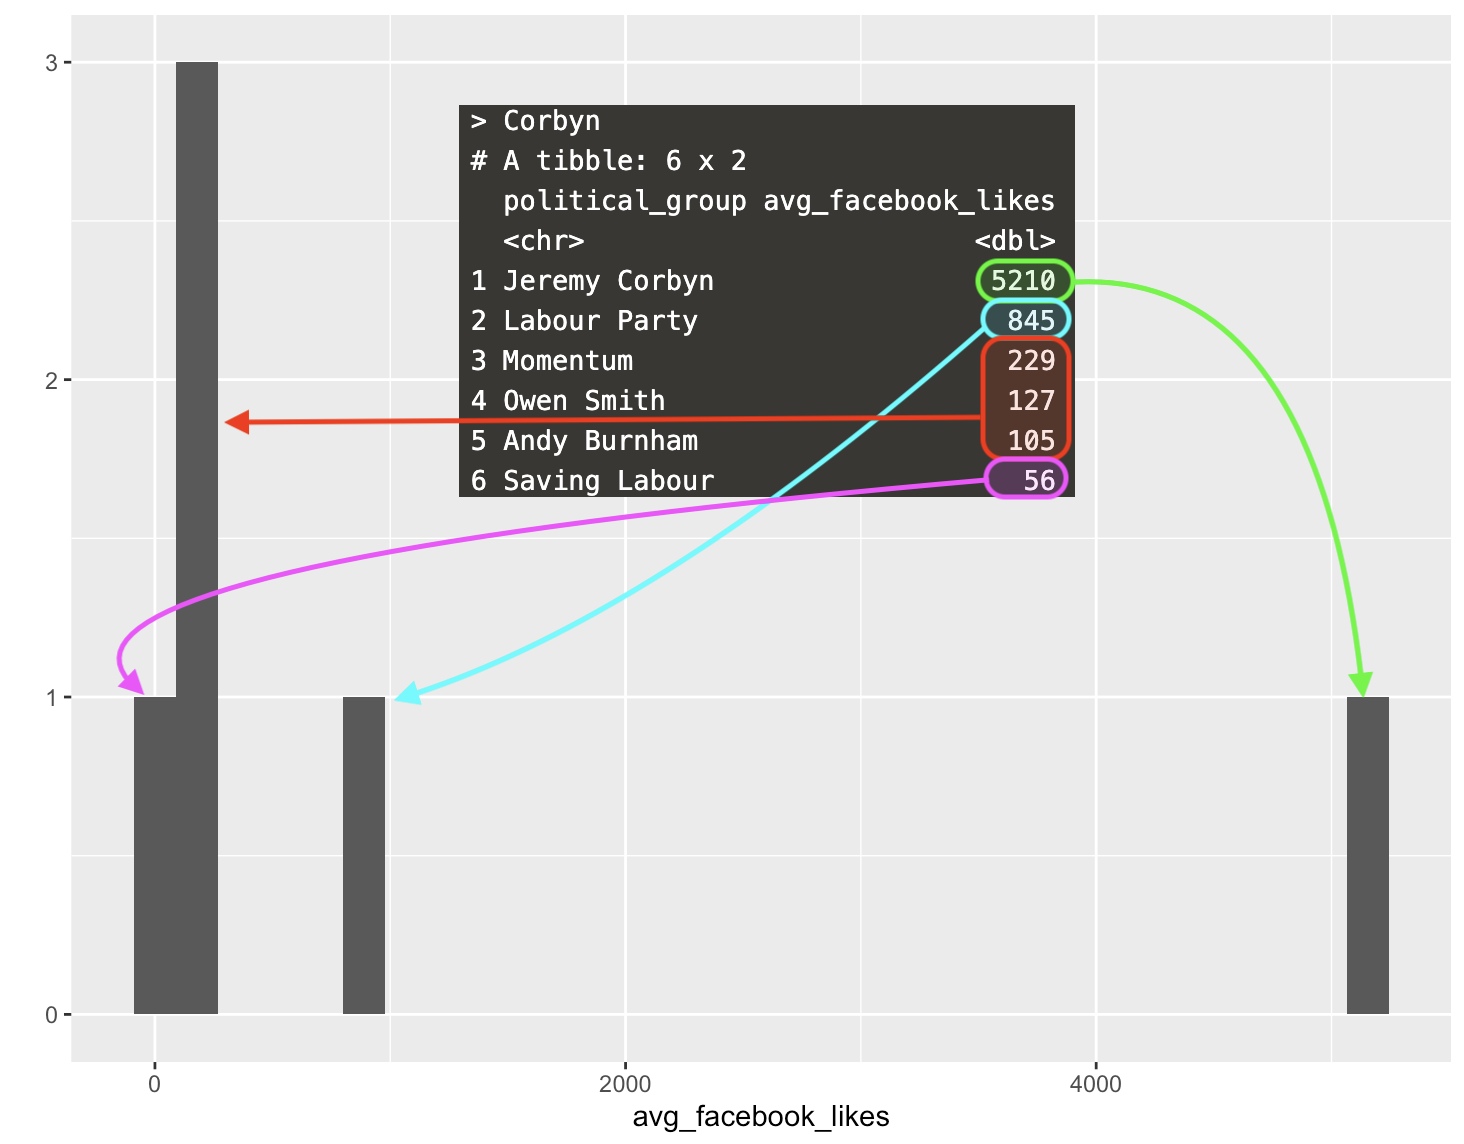
\includegraphics[width=7in,height=5in]{../img/corbyn-histogram} \end{center}

\hypertarget{visualize-a-single-variable-box-plots}{%
\section{Visualize a single variable:
box-plots}\label{visualize-a-single-variable-box-plots}}

Histograms are a great way to visualize the distribution of a single
variable, but there are other \texttt{geom}s, too. For example, a
box-plot gives us a graph with quite a few summary statistics.

The code section below will create a box-plot of the
\texttt{pop\_65\_percent} from the \texttt{Pensions} dataset.

\begin{Shaded}
\begin{Highlighting}[]
\NormalTok{Pensions }\SpecialCharTok{\%\textgreater{}\%} 
  \CommentTok{\# the variable }
\NormalTok{  ggplot2}\SpecialCharTok{::}\FunctionTok{qplot}\NormalTok{(}\AttributeTok{x =}\NormalTok{ pop\_65\_percent, }
                 \AttributeTok{y =} \StringTok{" "}\NormalTok{,}
                 \CommentTok{\# the dot}
                 \AttributeTok{data =}\NormalTok{ .,}
                 \AttributeTok{geom =} \StringTok{"boxplot"}\NormalTok{)}
\end{Highlighting}
\end{Shaded}

\begin{center}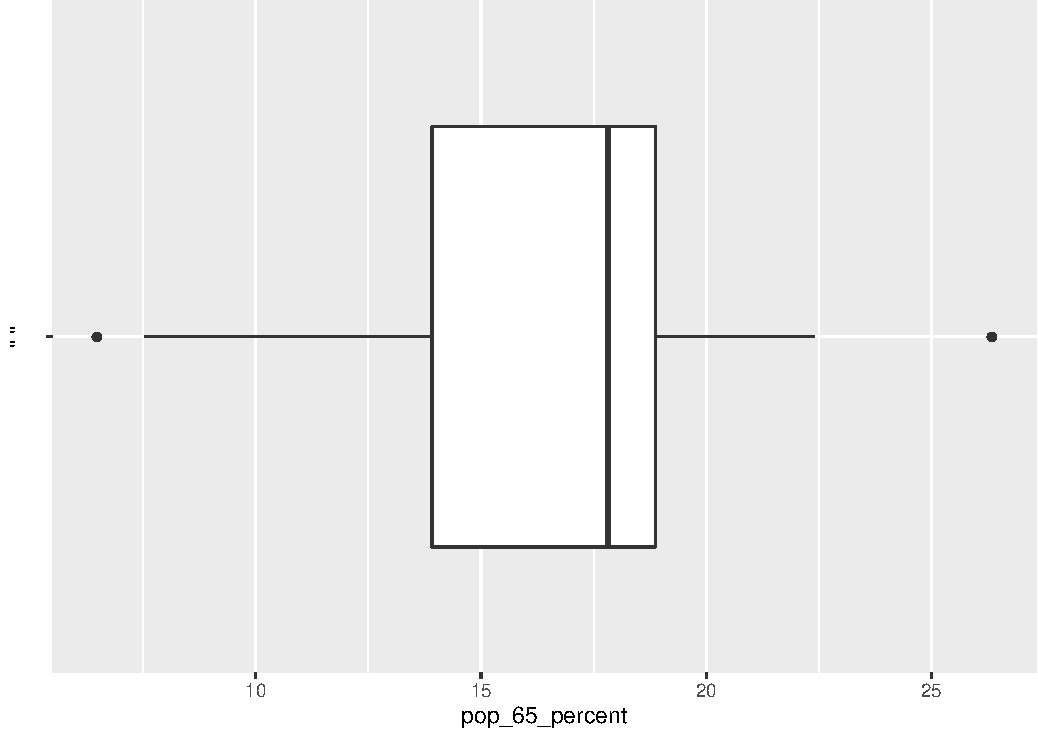
\includegraphics{03-intro-to-ggplot2_files/figure-latex/Pensions-boxplot-1} \end{center}

The box-plot gives us an idea of \texttt{pop\_65\_percent}'s
distribution using the white box to show where the median (middle
value), 1st and 3rd quartiles, higher/lower values, and outliers (see
image below).

\begin{center}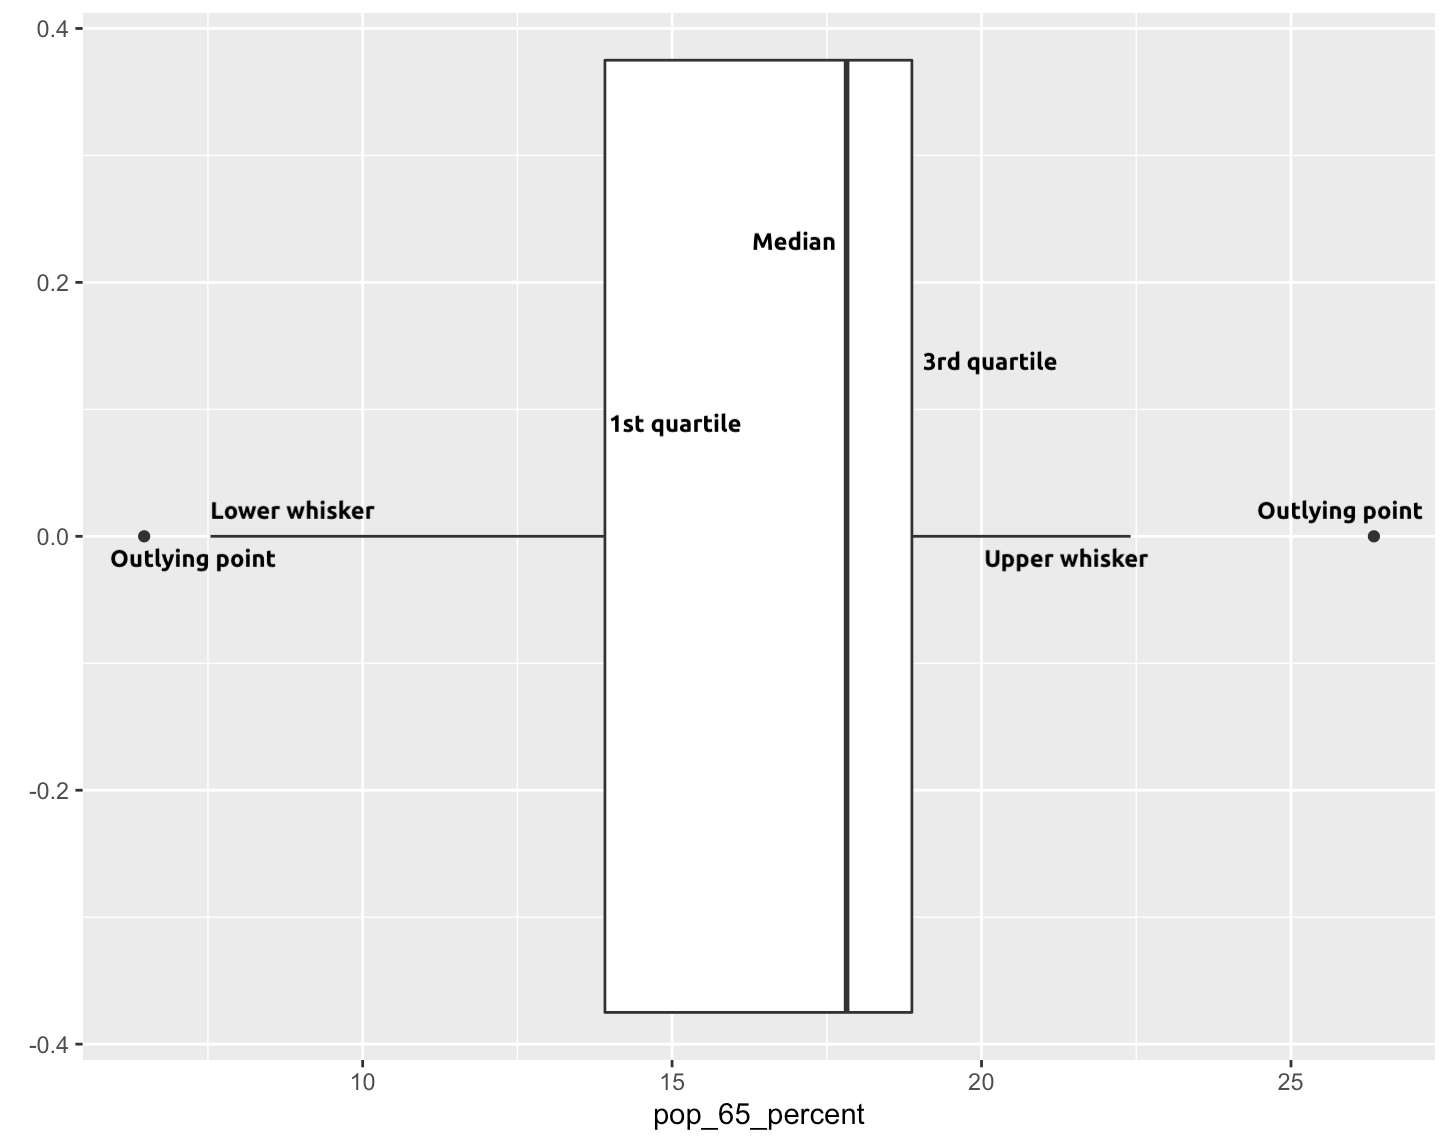
\includegraphics[width=5in,height=3.5in]{../img/pensions-boxplot} \end{center}

\hypertarget{visualizing-a-numerical-and-categorical-variable}{%
\section{Visualizing a numerical and categorical
variable}\label{visualizing-a-numerical-and-categorical-variable}}

Box-plots are also great for visualizing continuous variables across the
levels of a categorical variable. For example, we have the
\texttt{Balance} dataset with \texttt{value}s of European Union
countries' budget surplus. We can add the categorical variable to the
\texttt{y} axis to view one box-plot per \texttt{country} level.

\begin{Shaded}
\begin{Highlighting}[]
\CommentTok{\# the data}
\NormalTok{Balance }\SpecialCharTok{\%\textgreater{}\%} 
\NormalTok{  ggplot2}\SpecialCharTok{::}\FunctionTok{qplot}\NormalTok{(}\AttributeTok{x =}\NormalTok{ value, }\AttributeTok{y =}\NormalTok{ country, }
                 \AttributeTok{data =}\NormalTok{ ., }\AttributeTok{geom =} \StringTok{"boxplot"}\NormalTok{) }
\end{Highlighting}
\end{Shaded}

\begin{center}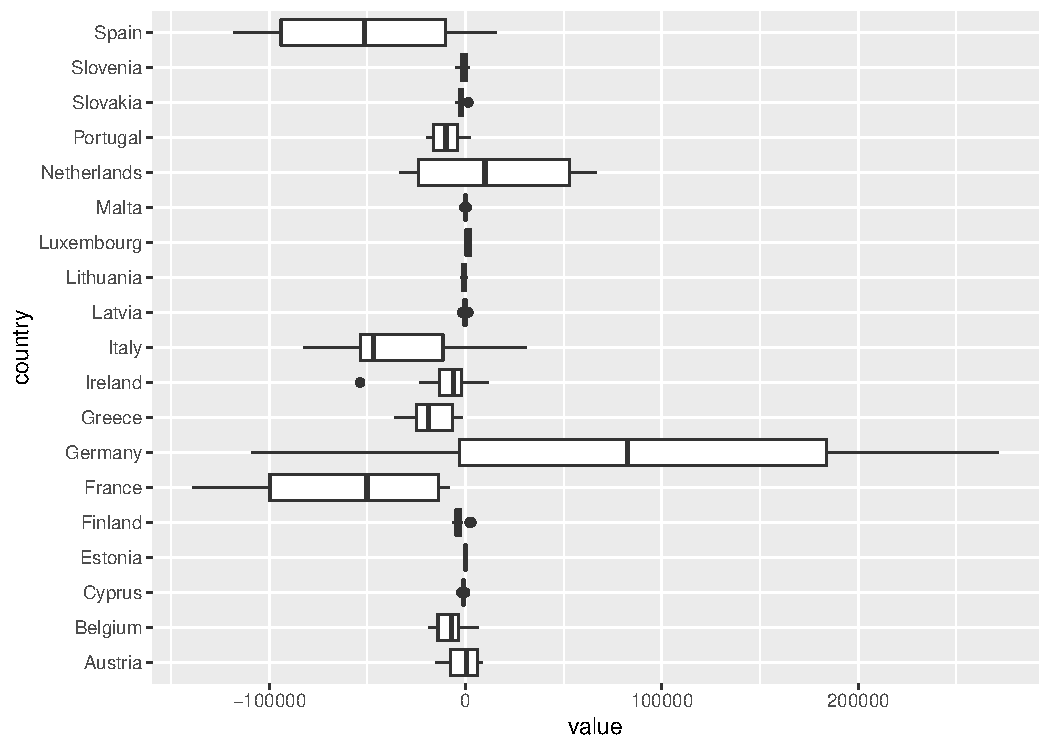
\includegraphics{03-intro-to-ggplot2_files/figure-latex/Balance-boxplot-country-value-1} \end{center}

Other options for individual variables include the
\href{https://ggplot2.tidyverse.org/reference/geom_density.html}{\texttt{geom\ =\ "density"}}
and
\href{https://ggplot2.tidyverse.org/reference/geom_violin.html}{\texttt{geom\ =\ "violin"}}.

\hypertarget{visualizing-two-continuous-variables}{%
\section{Visualizing two continuous
variables}\label{visualizing-two-continuous-variables}}

What if we want to graph the relationship between two variables? We'll
graph two variables from the \texttt{Brexit} dataset.

Use RStudio to view this dataset with \texttt{dplyr::glimpse()} or
\texttt{utils::str()}.

\begin{Shaded}
\begin{Highlighting}[]
\FunctionTok{glimpse}\NormalTok{(Brexit)}
\end{Highlighting}
\end{Shaded}

\begin{ShadedResult}
\begin{verbatim}
#  Rows: 85
#  Columns: 3
#  $ date                     <chr> "2/8/16", "9/8/16", "17/08/16", "23/08/16", "~
#  $ percent_responding_right <dbl> 46, 45, 46, 45, 47, 46, 45, 45, 46, 44, 44, 4~
#  $ percent_responding_wrong <dbl> 42, 44, 43, 43, 44, 43, 44, 44, 43, 45, 42, 4~
\end{verbatim}
\end{ShadedResult}

When we view the contents of \texttt{Brexit}, we can see the
\texttt{date} column is a character variable
(\texttt{\textless{}chr\textgreater{}}), and the other two
variables--\texttt{percent\_responding\_right} and
\texttt{percent\_responding\_wrong}--are numeric
(\texttt{\textless{}dbl\textgreater{}}).

\hypertarget{creating-date-variables}{%
\subsection{\texorpdfstring{\textbf{\emph{Creating date
variables}}}{Creating date variables}}\label{creating-date-variables}}

If we want to plot the relationship between \texttt{date} and the
\texttt{percent\_responding\_right}, we'll first need to change the
format of \texttt{date} from character to \texttt{Date}, which we can do
using the \href{https://lubridate.tidyverse.org/}{\texttt{lubridate}
package} (also from the \texttt{tidyverse}).

We use the \texttt{lubridate::mdy()} function to format the
\texttt{date} variable as a \texttt{Date}.

\begin{Shaded}
\begin{Highlighting}[]
\NormalTok{Brexit }\OtherTok{\textless{}{-}}\NormalTok{ Brexit }\SpecialCharTok{\%\textgreater{}\%} \FunctionTok{mutate}\NormalTok{(}\AttributeTok{date =}\NormalTok{ lubridate}\SpecialCharTok{::}\FunctionTok{dmy}\NormalTok{(date))}
\end{Highlighting}
\end{Shaded}

Read more about \texttt{dmy()}
\href{https://lubridate.tidyverse.org/reference/ymd.html}{here.}

Use the \texttt{base::is.double()}, \texttt{base::class()}, or
\texttt{base::typeof()} function to figure out if you've formatted the
new date variable correctly.

\begin{Shaded}
\begin{Highlighting}[]
\NormalTok{base}\SpecialCharTok{::}\FunctionTok{is.double}\NormalTok{(Brexit}\SpecialCharTok{$}\NormalTok{date)}
\end{Highlighting}
\end{Shaded}

\begin{ShadedResult}
\begin{verbatim}
#  [1] TRUE
\end{verbatim}
\end{ShadedResult}

\begin{Shaded}
\begin{Highlighting}[]
\NormalTok{base}\SpecialCharTok{::}\FunctionTok{class}\NormalTok{(Brexit}\SpecialCharTok{$}\NormalTok{date)}
\end{Highlighting}
\end{Shaded}

\begin{ShadedResult}
\begin{verbatim}
#  [1] "Date"
\end{verbatim}
\end{ShadedResult}

\begin{Shaded}
\begin{Highlighting}[]
\NormalTok{base}\SpecialCharTok{::}\FunctionTok{typeof}\NormalTok{(Brexit}\SpecialCharTok{$}\NormalTok{date)}
\end{Highlighting}
\end{Shaded}

\begin{ShadedResult}
\begin{verbatim}
#  [1] "double"
\end{verbatim}
\end{ShadedResult}

After we're sure we've formatted the \texttt{date} variable correctly,
we want to `pipe' the formatted data to the \texttt{ggplot2::qplot()}
function with the new \texttt{date} variable on the \texttt{x} and the
\texttt{percent\_responding\_right} variable on the \texttt{y}.

\begin{Shaded}
\begin{Highlighting}[]
\NormalTok{Brexit }\SpecialCharTok{\%\textgreater{}\%} 
  \FunctionTok{qplot}\NormalTok{(}\AttributeTok{x =}\NormalTok{ date, }
        \AttributeTok{y =}\NormalTok{ percent\_responding\_right, }\AttributeTok{data =}\NormalTok{ .)}
\end{Highlighting}
\end{Shaded}

\begin{center}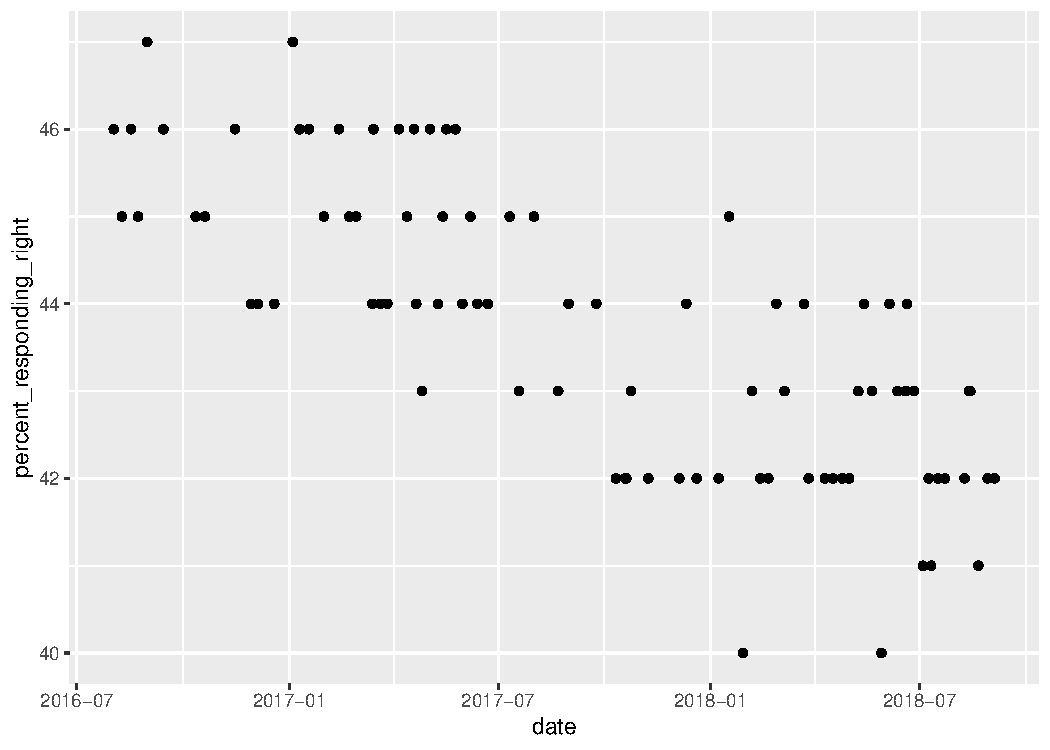
\includegraphics{03-intro-to-ggplot2_files/figure-latex/lubridate-date-1} \end{center}

The \texttt{ggplot2::qplot()} function is smart enough to automatically
choose a \texttt{geom} depending on what type of variable we assign to
the \texttt{x} and \texttt{y} axes. In this case, the
\texttt{percent\_responding\_right} variable is a
\texttt{\textless{}dbl\textgreater{}} (numeric), and we've reformatted
the \texttt{date} variable into a double before we passed it to the
\texttt{y} axis.

The \texttt{ggplot2::qplot()} function knows to plot the dates on the
\texttt{y} axes (notice it displays only the \texttt{year}) and
represent the data with \texttt{geom\ =\ "points"}.

\hypertarget{wrangling-and-visualization-pipelines}{%
\section{Wrangling and visualization
pipelines}\label{wrangling-and-visualization-pipelines}}

Sometimes we might want to pass the data directly from a wrangling step
to a data visualization without assigning changes to the data frame. We
will demonstrate how this works using the same \texttt{Brexit} dataset.

If you read the
\href{https://medium.economist.com/mistakes-weve-drawn-a-few-8cdd8a42d368}{Medium
article}, you'll find The Economist first plotted these data as a line
graph, with two lines (see `Original' image below). The `Better' way to
improve the graph would be to include points and smooth the line in the
graph (see below):

\begin{center}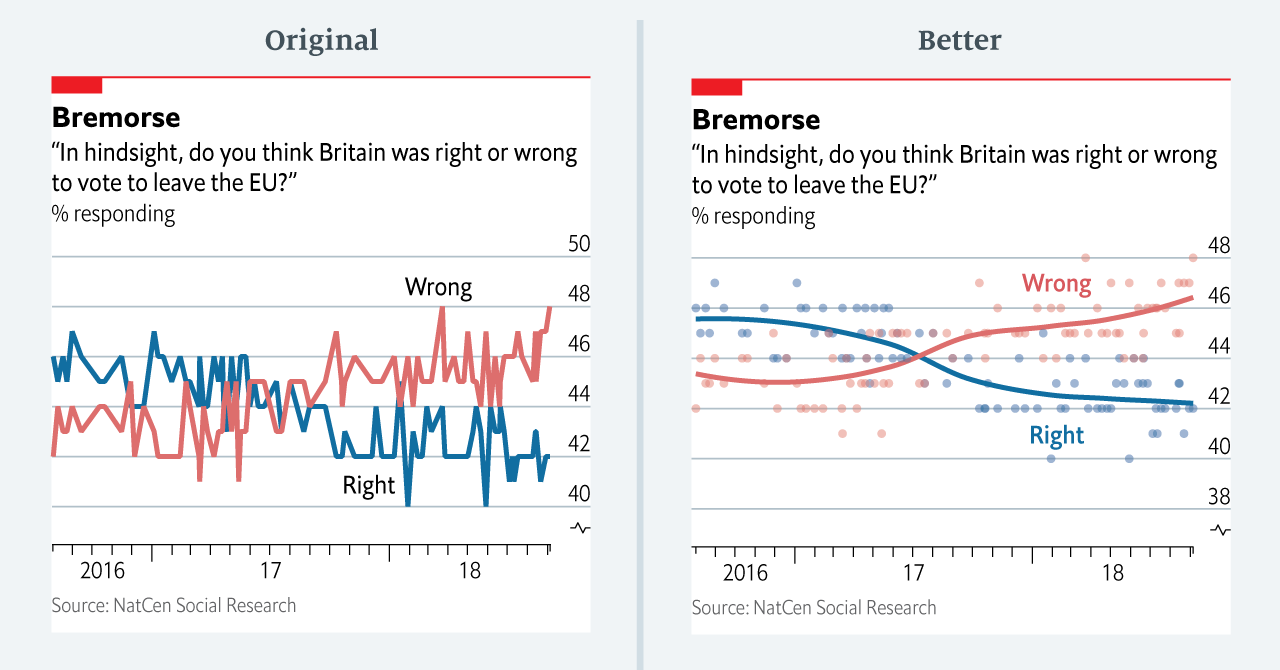
\includegraphics[width=7in,height=4in]{../img/original-brexit} \end{center}

In order to re-create these graphs, we'll need to restructure the
\texttt{Brexit} data with the \texttt{tidyr::pivot\_longer()} function
from the
\href{https://tidyr.tidyverse.org/reference/pivot_longer.html}{\texttt{tidyr}
package}.

We should end up with a dataset that has three variables: \texttt{date},
\texttt{poll}, and \texttt{percent}.

\begin{Shaded}
\begin{Highlighting}[]
\NormalTok{Brexit }\SpecialCharTok{\%\textgreater{}\%} \FunctionTok{pivot\_longer}\NormalTok{(}\AttributeTok{cols =} \SpecialCharTok{{-}}\NormalTok{date, }
                        \AttributeTok{names\_to =} \StringTok{"poll"}\NormalTok{, }
                        \AttributeTok{values\_to =} \StringTok{"percent"}\NormalTok{)}
\end{Highlighting}
\end{Shaded}

\begin{ShadedResult}
\begin{verbatim}
#  # A tibble: 170 x 3
#     date       poll                     percent
#     <date>     <chr>                      <dbl>
#   1 2016-08-02 percent_responding_right      46
#   2 2016-08-02 percent_responding_wrong      42
#   3 2016-08-09 percent_responding_right      45
#   4 2016-08-09 percent_responding_wrong      44
#   5 2016-08-17 percent_responding_right      46
#   6 2016-08-17 percent_responding_wrong      43
#   7 2016-08-23 percent_responding_right      45
#   8 2016-08-23 percent_responding_wrong      43
#   9 2016-08-31 percent_responding_right      47
#  10 2016-08-31 percent_responding_wrong      44
#  # ... with 160 more rows
\end{verbatim}
\end{ShadedResult}

\hypertarget{restructure-and-plot}{%
\subsection{\texorpdfstring{\textbf{\emph{Restructure and
plot}}}{Restructure and plot}}\label{restructure-and-plot}}

After we're sure the data are structured correctly, we won't assign it
to the \texttt{Brexit} data frame. Instead, we'll pass it straight
through to the \texttt{ggplot2::qplot()} function. The \texttt{date}
variable will go on the \texttt{x}, and the \texttt{percent} variable
will go on the \texttt{y}. Click on the Run icon below to see the graph.

First, we will create the `Original' graph by using
\texttt{group\ =\ poll} and \texttt{geom\ =\ "line\textquotesingle{}},
because this allows us to build a separate colored line for each
\texttt{poll}.

\begin{Shaded}
\begin{Highlighting}[]
\NormalTok{Brexit }\SpecialCharTok{\%\textgreater{}\%} 
  \FunctionTok{pivot\_longer}\NormalTok{(}\AttributeTok{cols =} \SpecialCharTok{{-}}\NormalTok{date, }
               \AttributeTok{names\_to =} \StringTok{"poll"}\NormalTok{, }
               \AttributeTok{values\_to =} \StringTok{"percent"}\NormalTok{) }\SpecialCharTok{\%\textgreater{}\%} 
\NormalTok{  ggplot2}\SpecialCharTok{::}\FunctionTok{qplot}\NormalTok{(}\AttributeTok{x =}\NormalTok{ date, }
                 \AttributeTok{y =}\NormalTok{ percent,}
                 \AttributeTok{group =}\NormalTok{ poll,}
                 \AttributeTok{data =}\NormalTok{ .,}
                 \AttributeTok{geom =} \StringTok{"line"}\NormalTok{,}
                 \AttributeTok{color =}\NormalTok{ poll)}
\end{Highlighting}
\end{Shaded}

\begin{center}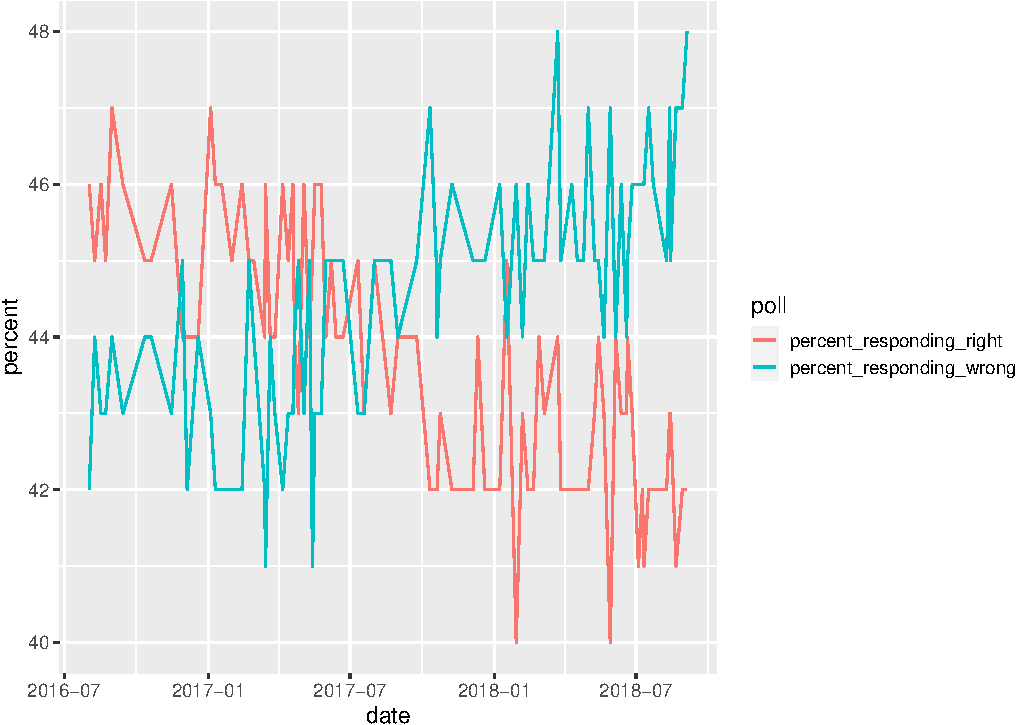
\includegraphics{03-intro-to-ggplot2_files/figure-latex/pivot_longer-qplot-1} \end{center}

As we can see from the graph above, using \texttt{group} and the
\texttt{color} aesthetic extends the \texttt{qplot()}'s capabilities by
making it clear there are two categories for \texttt{polls} represented
in the graph.

\hypertarget{build-plots-layer-by-layer-with-ggplot}{%
\subsection{\texorpdfstring{\textbf{\emph{Build plots layer-by-layer
with
\texttt{ggplot()}}}}{Build plots layer-by-layer with ggplot()}}\label{build-plots-layer-by-layer-with-ggplot}}

Now that we've learned how to plot using geoms and aesthetics, we can
add layers to the graph. In the previous step, we re-created the
`Original' plot using \texttt{geom\ =\ "line"}. The
\texttt{ggplot2::qplot()} function was written to ``produce plots
quickly'', but more complex graphs should be built using the
\texttt{ggplot2::ggplot()} function.

The \texttt{ggplot2::ggplot()} function initializes a graph, then we can
`map' variables to the positions (\texttt{x} or \texttt{y}), aesthetics
(\texttt{color\ =}), or groupings (\texttt{group\ =}).

We'll start by assigning the restructuring changes to the
\texttt{Brexit} dataset. The \texttt{tidyr::pivot\_longer()} function
takes a `wide' dataset and makes it `long', or
\href{https://vita.had.co.nz/papers/tidy-data.pdf}{tidy}.

We will store the restructured data in \texttt{TidyBrexit}.

\begin{Shaded}
\begin{Highlighting}[]
\NormalTok{TidyBrexit }\OtherTok{\textless{}{-}}\NormalTok{ Brexit }\SpecialCharTok{\%\textgreater{}\%} \FunctionTok{pivot\_longer}\NormalTok{(}\SpecialCharTok{{-}}\NormalTok{date, }
                                  \AttributeTok{names\_to =} \StringTok{"poll"}\NormalTok{, }
                                  \AttributeTok{values\_to =} \StringTok{"percent"}\NormalTok{)}
\FunctionTok{head}\NormalTok{(TidyBrexit)}
\end{Highlighting}
\end{Shaded}

\begin{ShadedResult}
\begin{verbatim}
#  # A tibble: 6 x 3
#    date       poll                     percent
#    <date>     <chr>                      <dbl>
#  1 2016-08-02 percent_responding_right      46
#  2 2016-08-02 percent_responding_wrong      42
#  3 2016-08-09 percent_responding_right      45
#  4 2016-08-09 percent_responding_wrong      44
#  5 2016-08-17 percent_responding_right      46
#  6 2016-08-17 percent_responding_wrong      43
\end{verbatim}
\end{ShadedResult}

\hypertarget{using-the-ggplot-function}{%
\section{\texorpdfstring{Using the \texttt{ggplot()}
function}{Using the ggplot() function}}\label{using-the-ggplot-function}}

The \texttt{ggplot()} follows a pretty standard template, similar to the
\texttt{qplot()} function. See below:

\begin{Shaded}
\begin{Highlighting}[]
\SpecialCharTok{\textless{}}\NormalTok{DATA}\SpecialCharTok{\textgreater{}} \SpecialCharTok{\%\textgreater{}\%} 
  \FunctionTok{ggplot}\NormalTok{(}\AttributeTok{mapping =} \FunctionTok{aes}\NormalTok{(}\AttributeTok{x =} \SpecialCharTok{\textless{}}\NormalTok{MAPPINGS}\SpecialCharTok{\textgreater{}}\NormalTok{, }\AttributeTok{y =} \SpecialCharTok{\textless{}}\NormalTok{MAPPINGS}\SpecialCharTok{\textgreater{}}\NormalTok{))}
\end{Highlighting}
\end{Shaded}

We begin with a dataset, pass it over to to the \texttt{ggplot()}
function, then map the \texttt{x} and \texttt{y} variables.

\begin{Shaded}
\begin{Highlighting}[]
\NormalTok{ggp\_brexit }\OtherTok{\textless{}{-}}\NormalTok{ TidyBrexit }\SpecialCharTok{\%\textgreater{}\%} \FunctionTok{ggplot}\NormalTok{(}\AttributeTok{mapping =} \FunctionTok{aes}\NormalTok{(}\AttributeTok{x =}\NormalTok{ date, }\AttributeTok{y =}\NormalTok{ percent))}
\NormalTok{ggp\_brexit}
\end{Highlighting}
\end{Shaded}

\begin{center}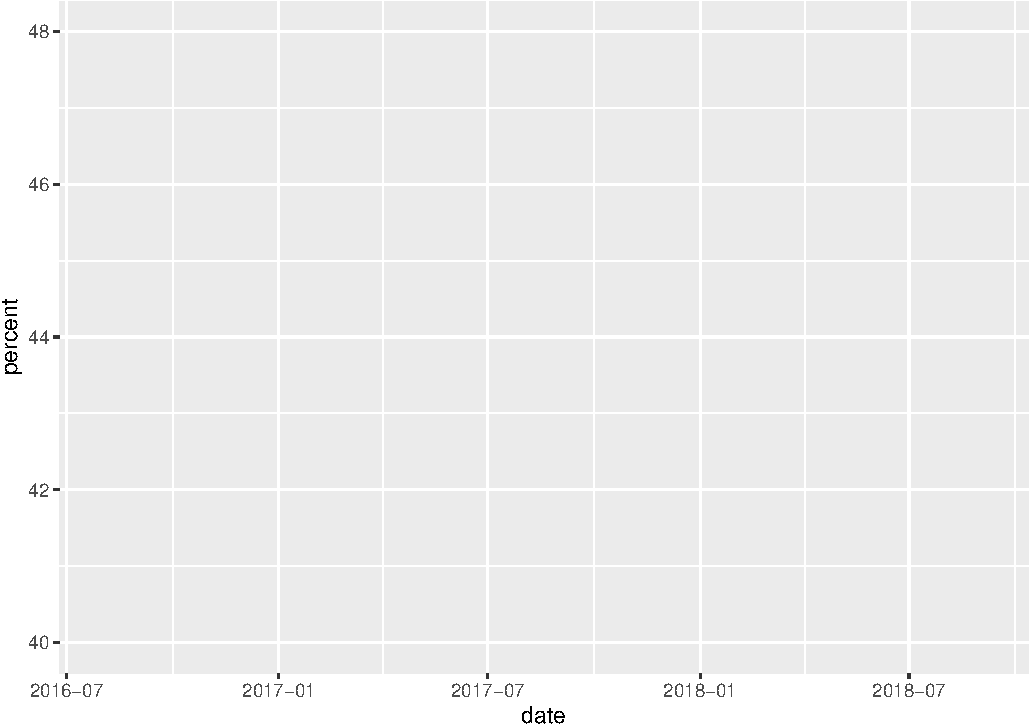
\includegraphics{03-intro-to-ggplot2_files/figure-latex/TidyBrexit-ggplot-1} \end{center}

There aren't any points on the graph because we haven't added any geoms
or aesthetics.

We'll add the smoothed line in the step below with
\texttt{ggplot2::geom\_smooth()} like the template below.

\begin{Shaded}
\begin{Highlighting}[]
\SpecialCharTok{\textless{}}\NormalTok{DATA}\SpecialCharTok{\textgreater{}} \SpecialCharTok{\%\textgreater{}\%} 
  \FunctionTok{ggplot}\NormalTok{(}\AttributeTok{mapping =} \FunctionTok{aes}\NormalTok{(}\AttributeTok{x =} \SpecialCharTok{\textless{}}\NormalTok{MAPPINGS}\SpecialCharTok{\textgreater{}}\NormalTok{, }\AttributeTok{y =} \SpecialCharTok{\textless{}}\NormalTok{MAPPINGS}\SpecialCharTok{\textgreater{}}\NormalTok{)) }\SpecialCharTok{+} 
    \ErrorTok{\textless{}}\NormalTok{GEOM\_FUNCTION}\SpecialCharTok{\textgreater{}}\NormalTok{(}\AttributeTok{mapping =} \FunctionTok{aes}\NormalTok{(}\SpecialCharTok{\textless{}}\NormalTok{MAPPINGS}\SpecialCharTok{\textgreater{}}\NormalTok{))}
\end{Highlighting}
\end{Shaded}

\textbf{Note}: the \texttt{+} operator is used with \texttt{ggplot2}
functions, not the pipe \texttt{\%\textgreater{}\%} operator.

\begin{Shaded}
\begin{Highlighting}[]
\NormalTok{ggp\_brexit }\SpecialCharTok{+}\NormalTok{ ggplot2}\SpecialCharTok{::}\FunctionTok{geom\_smooth}\NormalTok{()}
\end{Highlighting}
\end{Shaded}

\begin{center}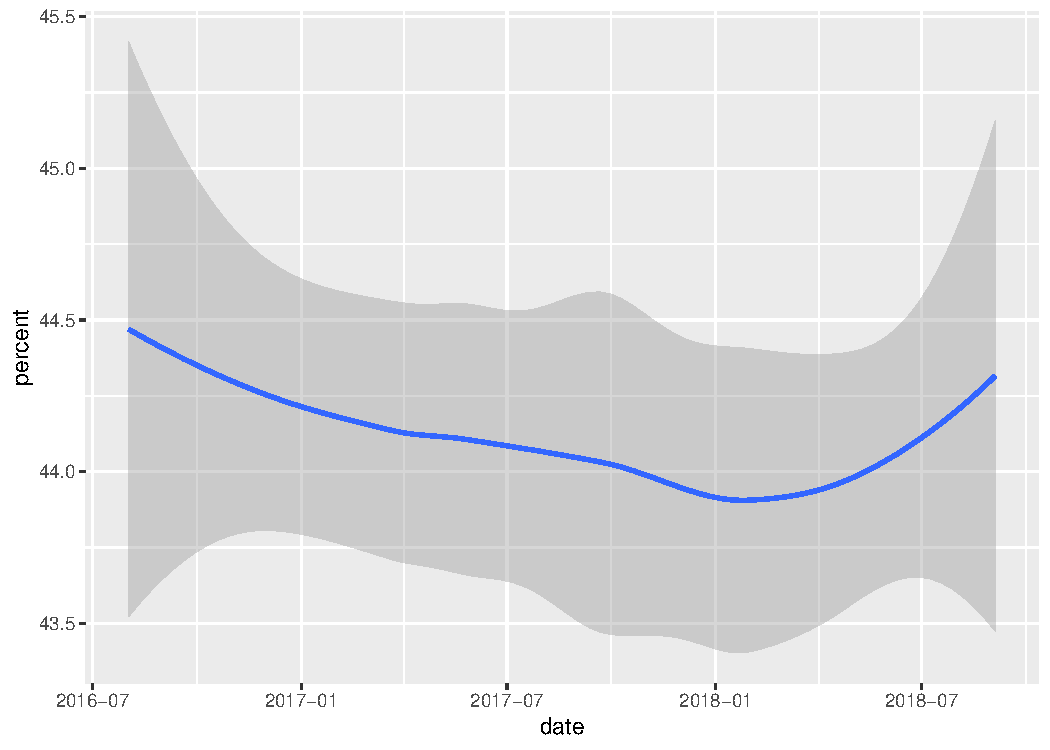
\includegraphics{03-intro-to-ggplot2_files/figure-latex/geom_smooth-1} \end{center}

\emph{Why are we only seeing a single line?} We need to look at our
template again:

\begin{Shaded}
\begin{Highlighting}[]
\SpecialCharTok{\textless{}}\NormalTok{DATA}\SpecialCharTok{\textgreater{}} \SpecialCharTok{\%\textgreater{}\%} 
  \FunctionTok{ggplot}\NormalTok{(}\AttributeTok{mapping =} \FunctionTok{aes}\NormalTok{(}\AttributeTok{x =} \SpecialCharTok{\textless{}}\NormalTok{MAPPINGS}\SpecialCharTok{\textgreater{}}\NormalTok{, }\AttributeTok{y =} \SpecialCharTok{\textless{}}\NormalTok{MAPPINGS}\SpecialCharTok{\textgreater{}}\NormalTok{)) }\SpecialCharTok{+} 
    \ErrorTok{\textless{}}\NormalTok{GEOM\_FUNCTION}\SpecialCharTok{\textgreater{}}\NormalTok{(}\AttributeTok{mapping =} \FunctionTok{aes}\NormalTok{(}\SpecialCharTok{\textless{}}\NormalTok{MAPPINGS}\SpecialCharTok{\textgreater{}}\NormalTok{))}
\end{Highlighting}
\end{Shaded}

We can see from the template above that we can set the aesthetic
mappings (\texttt{aes(\textless{}MAPPINGS\textgreater{})}) globally
\emph{and} inside the geom layer we want to display.

In this case, we want the lines from \texttt{geom\_smooth()} colored by
the two kinds of polls. We can set this with \texttt{color\ =\ poll}.

\begin{Shaded}
\begin{Highlighting}[]
\NormalTok{ggp\_brexit }\SpecialCharTok{+} 
\NormalTok{  ggplot2}\SpecialCharTok{::}\FunctionTok{geom\_smooth}\NormalTok{(}\FunctionTok{aes}\NormalTok{(}\AttributeTok{color =}\NormalTok{ poll))}
\end{Highlighting}
\end{Shaded}

\begin{center}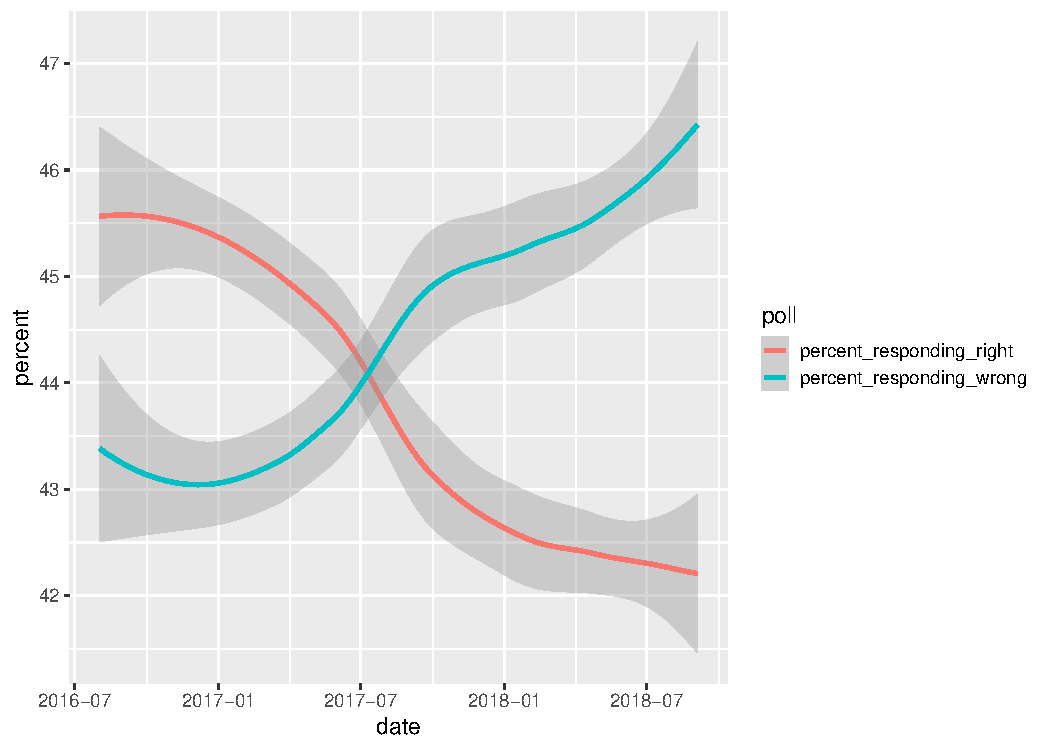
\includegraphics{03-intro-to-ggplot2_files/figure-latex/color-poll-1} \end{center}

The default \texttt{ggplot2::geom\_smooth()} function includes the gray
confidence interval around the smoothed line. We can remove this with
\texttt{se\ =\ FALSE}. We'll also add the \texttt{show.legend\ =\ FALSE}
argument to remove the \texttt{poll} categories from the left-hand side
of the graph.

\begin{Shaded}
\begin{Highlighting}[]
\NormalTok{ggp\_brexit\_smooth }\OtherTok{\textless{}{-}}\NormalTok{ ggp\_brexit }\SpecialCharTok{+} 
  \FunctionTok{geom\_smooth}\NormalTok{(}\FunctionTok{aes}\NormalTok{(}\AttributeTok{color =}\NormalTok{ poll), }\AttributeTok{se =} \ConstantTok{FALSE}\NormalTok{, }\AttributeTok{show.legend =} \ConstantTok{FALSE}\NormalTok{)}
\NormalTok{ggp\_brexit\_smooth}
\end{Highlighting}
\end{Shaded}

\begin{center}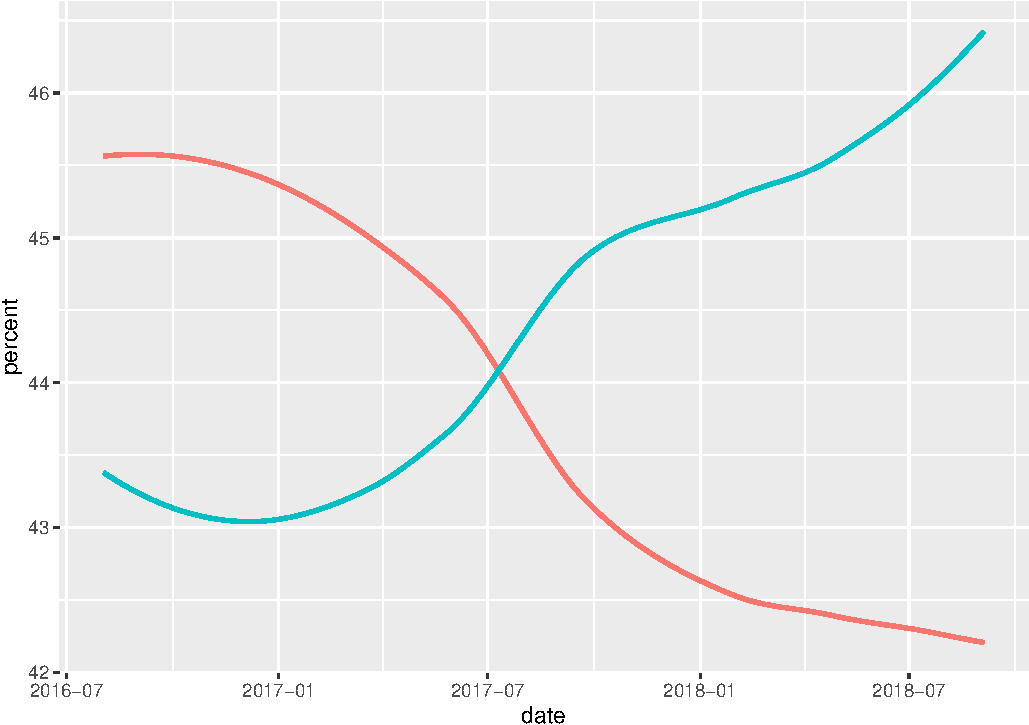
\includegraphics{03-intro-to-ggplot2_files/figure-latex/ggp_brexit_smooth-1} \end{center}

In the next step, we'll add the points to the graph. We've also updated
the template below for adding aesthetics.

\begin{Shaded}
\begin{Highlighting}[]
\SpecialCharTok{\textless{}}\NormalTok{DATA}\SpecialCharTok{\textgreater{}} \SpecialCharTok{\%\textgreater{}\%} 
  \FunctionTok{ggplot}\NormalTok{(}\AttributeTok{mapping =} \FunctionTok{aes}\NormalTok{(}\AttributeTok{x =} \SpecialCharTok{\textless{}}\NormalTok{MAPPINGS}\SpecialCharTok{\textgreater{}}\NormalTok{, }\AttributeTok{y =} \SpecialCharTok{\textless{}}\NormalTok{MAPPINGS}\SpecialCharTok{\textgreater{}}\NormalTok{)) }\SpecialCharTok{+} 
    \ErrorTok{\textless{}}\NormalTok{GEOM\_FUNCTION}\SpecialCharTok{\textgreater{}}\NormalTok{(}\AttributeTok{mapping =} \FunctionTok{aes}\NormalTok{(}\SpecialCharTok{\textless{}}\NormalTok{MAPPINGS}\SpecialCharTok{\textgreater{}}\NormalTok{), }
                    \AttributeTok{optional\_arguments =} \StringTok{"values"}\NormalTok{)}
\end{Highlighting}
\end{Shaded}

In the last step we added a \texttt{geom\_smooth()} removed the standard
errors (\texttt{se\ =\ FALSE}) and legend
(\texttt{show.legend\ =\ FALSE}). We stored these changes in the
\texttt{ggp\_brexit\_smooth}.

Refer to the template below for a refresher.

\begin{verbatim}
<DATA> %>% 
  ggplot(mapping = aes(x = <MAPPINGS>, y = <MAPPINGS>)) + 
    <GEOM_FUNCTION>(mapping = aes(<MAPPINGS>), 
                    optional_arguments = "values")
\end{verbatim}

We're going to continue building our plot by adding the
\texttt{ggplot2::geom\_point()} function. We need to specify the
\texttt{aes()} argument (\texttt{color\ =\ poll}), and we'll also
include the \texttt{show.legend\ =\ FALSE} argument again to remove the
legend for the two \texttt{poll} categories.

\begin{Shaded}
\begin{Highlighting}[]
\NormalTok{ggp\_brexit\_smooth }\SpecialCharTok{+} \FunctionTok{geom\_point}\NormalTok{(}\FunctionTok{aes}\NormalTok{(}\AttributeTok{color =}\NormalTok{ poll), }\AttributeTok{show.legend =} \ConstantTok{FALSE}\NormalTok{)}
\end{Highlighting}
\end{Shaded}

\begin{center}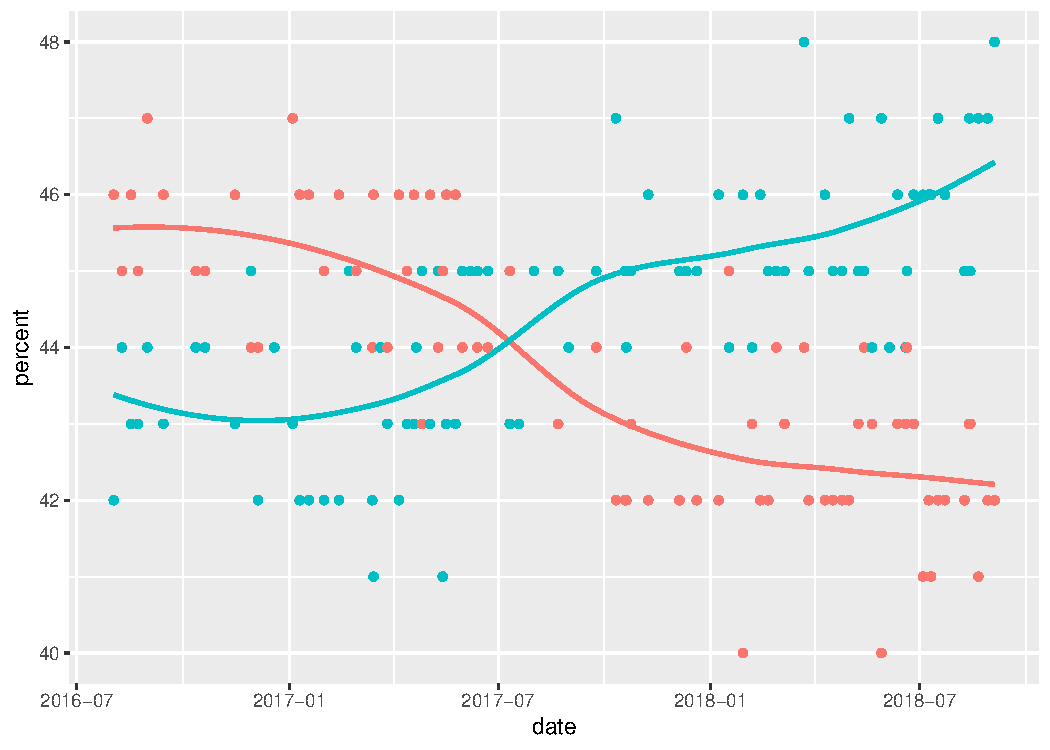
\includegraphics{03-intro-to-ggplot2_files/figure-latex/geom_point-1} \end{center}

This is starting to look more like the graph in the medium article, but
we still need to make a few minor adjustments.

\texttt{ggplot2} allows us to build graphs layer-by-layer using the
geoms and aesthetics to customize each plot so that they are necessarily
expressive. Each time we need to add something to a graph, we can either
add a new \texttt{geom}, or look for ways to adjust a geoms with new
aesthetic options.

For example, from the `Original' graph in the medium article, the points
are slightly transparent. The \texttt{alpha} is the transparency
argument, and it's available inside nearly every \texttt{geom}.

\begin{center}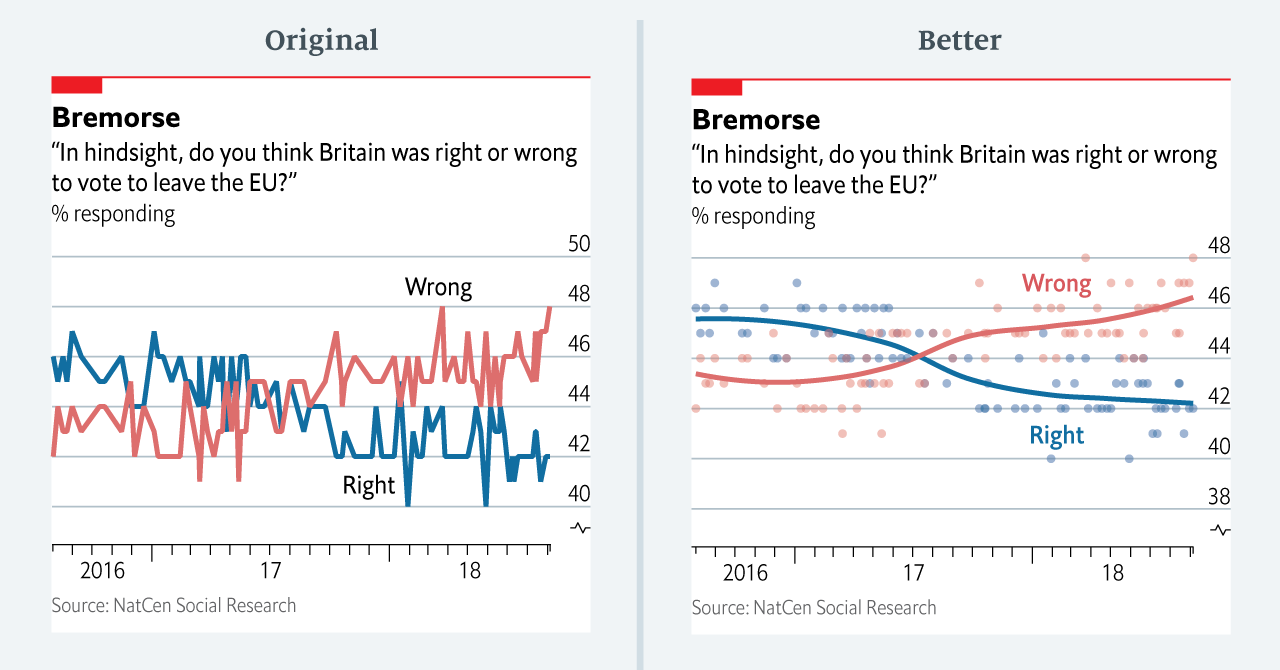
\includegraphics[width=7in,height=4in]{../img/original-brexit} \end{center}

We can add the \texttt{alpha} argument inside the
\texttt{ggplot2::geom\_point()} function, and specify either a decimal,
fraction, or numeric value. In this case, we want the value set to
\texttt{1/3}.

\begin{Shaded}
\begin{Highlighting}[]
\NormalTok{ggp\_brexit\_smooth }\SpecialCharTok{+} 
  \FunctionTok{geom\_point}\NormalTok{(}\FunctionTok{aes}\NormalTok{(}\AttributeTok{color =}\NormalTok{ poll), }\AttributeTok{show.legend =} \ConstantTok{FALSE}\NormalTok{, }\AttributeTok{alpha =} \DecValTok{1}\SpecialCharTok{/}\DecValTok{3}\NormalTok{)}
\end{Highlighting}
\end{Shaded}

\begin{center}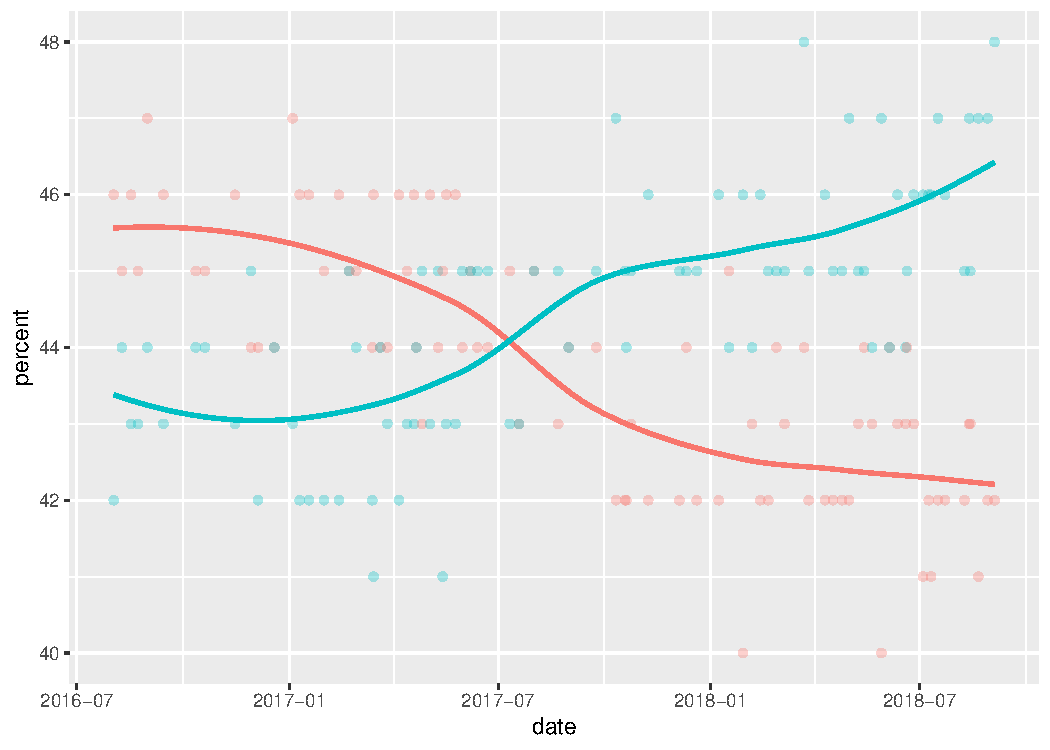
\includegraphics{03-intro-to-ggplot2_files/figure-latex/geom_point-alpha-1} \end{center}

Now the points are slightly transparent, which helps with over-plotting.
Review the template below for adding layers.

\begin{Shaded}
\begin{Highlighting}[]
\SpecialCharTok{\textless{}}\NormalTok{DATA}\SpecialCharTok{\textgreater{}} \SpecialCharTok{\%\textgreater{}\%} 
  \FunctionTok{ggplot}\NormalTok{(}\AttributeTok{mapping =} \FunctionTok{aes}\NormalTok{(}\AttributeTok{x =} \SpecialCharTok{\textless{}}\NormalTok{MAPPINGS}\SpecialCharTok{\textgreater{}}\NormalTok{, }\AttributeTok{y =} \SpecialCharTok{\textless{}}\NormalTok{MAPPINGS}\SpecialCharTok{\textgreater{}}\NormalTok{)) }\SpecialCharTok{+} 
    \ErrorTok{\textless{}}\NormalTok{GEOM\_FUNCTION}\SpecialCharTok{\textgreater{}}\NormalTok{(}\AttributeTok{mapping =} \FunctionTok{aes}\NormalTok{(}\SpecialCharTok{\textless{}}\NormalTok{MAPPINGS}\SpecialCharTok{\textgreater{}}\NormalTok{), }\AttributeTok{args =} \StringTok{"options"}\NormalTok{)}
\end{Highlighting}
\end{Shaded}

As you can see, the grammar of graphics makes it easy to think about
what we'd like to see on a plot, decide what kind of graph element it is
(\texttt{geom}, \texttt{aesthetic}, etc.), and then add it as a layer
with the \texttt{+} operator. Hopefully, you can see how easy it is to
customize a graph by adding new layers and aesthetics!

\hypertarget{mapping-aesthetics-globally}{%
\section{Mapping aesthetics
globally}\label{mapping-aesthetics-globally}}

\textbf{Note}: so far, we have added the \texttt{aes()} arguments
\emph{locally} in each new \texttt{geom} layer we've built. This section
will map these variables \emph{globally} in the \texttt{ggplot()}
function. See the code below:

\begin{Shaded}
\begin{Highlighting}[]
\NormalTok{ggp\_brexit\_global }\OtherTok{\textless{}{-}}\NormalTok{ TidyBrexit }\SpecialCharTok{\%\textgreater{}\%} 
  \FunctionTok{ggplot}\NormalTok{(}\AttributeTok{mapping =} \FunctionTok{aes}\NormalTok{(}\AttributeTok{x =}\NormalTok{ date, }\AttributeTok{y =}\NormalTok{ percent, }\AttributeTok{color =}\NormalTok{ poll)) }\SpecialCharTok{+} 
              \FunctionTok{geom\_smooth}\NormalTok{(}\AttributeTok{se =} \ConstantTok{FALSE}\NormalTok{, }\AttributeTok{show.legend =} \ConstantTok{FALSE}\NormalTok{) }\SpecialCharTok{+} 
                \FunctionTok{geom\_point}\NormalTok{(}\AttributeTok{alpha =} \DecValTok{1}\SpecialCharTok{/}\DecValTok{3}\NormalTok{, }\AttributeTok{show.legend =} \ConstantTok{FALSE}\NormalTok{)}
\NormalTok{ggp\_brexit\_global}
\end{Highlighting}
\end{Shaded}

\begin{center}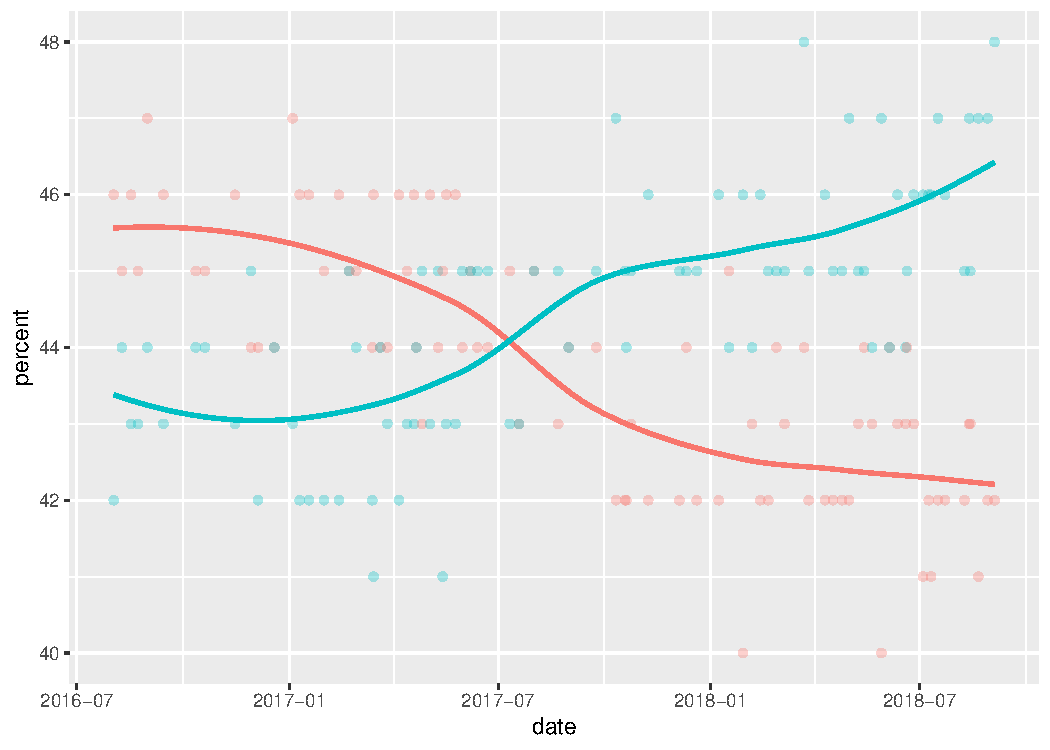
\includegraphics{03-intro-to-ggplot2_files/figure-latex/ggp_brexit_global-1} \end{center}

By adding \texttt{color\ =\ poll} in the \texttt{ggplot()} function, the
aesthetic carries down through each \texttt{geom}. All we have to do is
add the arguments for each \texttt{geom}.

\hypertarget{adding-colors-manually}{%
\subsection{\texorpdfstring{\textbf{\emph{Adding colors
manually}}}{Adding colors manually}}\label{adding-colors-manually}}

We want to change the graph's colors from the default settings to
fire-brick red and cornflower blue. We can do this by adding the
\texttt{ggplot2::scale\_color\_manual()} function and specifying the
values(\texttt{c("cornflowerblue",\ "firebrick3")}).

\begin{Shaded}
\begin{Highlighting}[]
\NormalTok{ggp\_brexit\_global\_colors }\OtherTok{\textless{}{-}}\NormalTok{ ggp\_brexit\_global }\SpecialCharTok{+}  
  \FunctionTok{scale\_color\_manual}\NormalTok{(}\AttributeTok{values =} \FunctionTok{c}\NormalTok{(}\StringTok{"cornflowerblue"}\NormalTok{, }\StringTok{"firebrick3"}\NormalTok{))}
\NormalTok{ggp\_brexit\_global\_colors}
\end{Highlighting}
\end{Shaded}

\begin{center}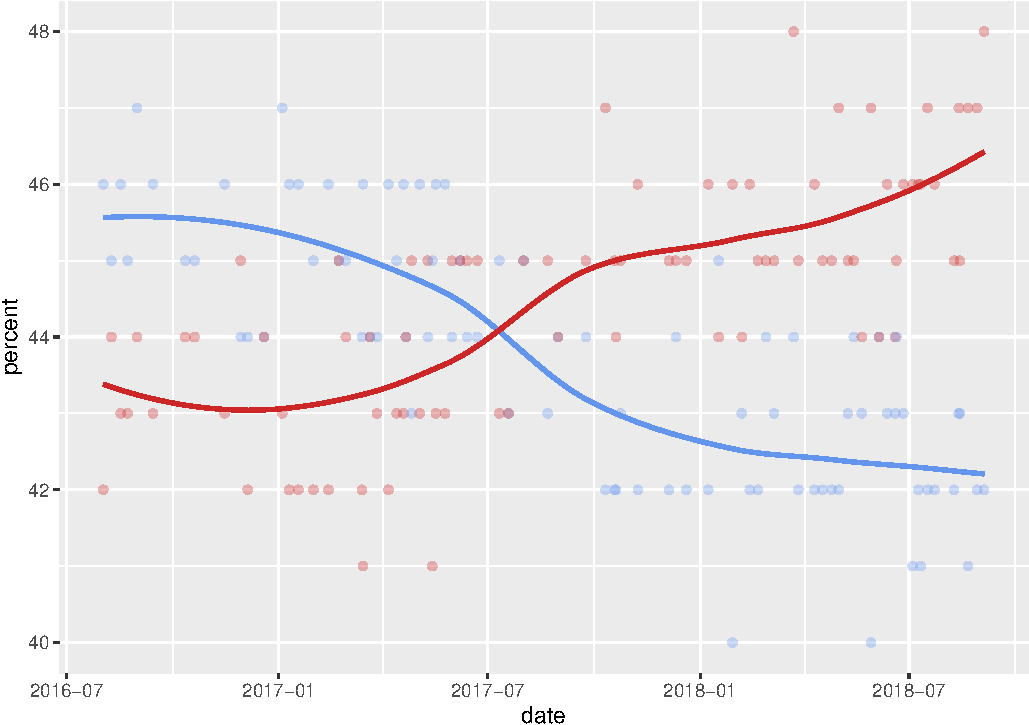
\includegraphics{03-intro-to-ggplot2_files/figure-latex/scale_color_manual-1} \end{center}

For a full list of colors, check the pdf
\href{http://www.stat.columbia.edu/~tzheng/files/Rcolor.pdf}{here}.

\hypertarget{adding-text-to-a-graph}{%
\subsection{\texorpdfstring{\textbf{\emph{Adding text to a
graph}}}{Adding text to a graph}}\label{adding-text-to-a-graph}}

In the
\href{https://medium.economist.com/mistakes-weve-drawn-a-few-8cdd8a42d368}{Medium
article}, the fixed `Better' graph labels each smoothed line with
\texttt{\textquotesingle{}Wrong\textquotesingle{}} vs
\texttt{\textquotesingle{}Right\textquotesingle{}}.

We're going to add text labels to our graph using the
\texttt{ggplot2::geom\_text()} function. The
\texttt{ggp\_brexit\_global\_colors} object has the latest changes to
the plot.

\hypertarget{using-the-geom_text-function}{%
\subsection{\texorpdfstring{\textbf{\emph{Using the
\texttt{geom\_text()}
function}}}{Using the geom\_text() function}}\label{using-the-geom_text-function}}

\texttt{ggplot2::geom\_text()} works on a Cartesian coordinate system
and requires the \texttt{x}, \texttt{y}, and \texttt{label} arguments.
We want to place the \texttt{Wrong} label at the intersection of percent
\texttt{46}, just above the red line near the year \texttt{2018}.

Recall that the dates are formatted as \texttt{YYYY-MM-DD}, so we have
to pick an \texttt{x} value that we can specify as a date with
\texttt{as.Date()}. See the example below:

\begin{Shaded}
\begin{Highlighting}[]
\NormalTok{ggp\_brexit\_global\_colors }\SpecialCharTok{+} 
  \FunctionTok{geom\_text}\NormalTok{(}\AttributeTok{label =} \StringTok{"Wrong"}\NormalTok{, }\AttributeTok{color =} \StringTok{"firebrick3"}\NormalTok{, }
            \AttributeTok{x =} \FunctionTok{as.Date}\NormalTok{(}\StringTok{"2018{-}01{-}01"}\NormalTok{), }\AttributeTok{y =} \DecValTok{46}\NormalTok{)}
\end{Highlighting}
\end{Shaded}

Now we want to add the \texttt{Right} label to the graph, but make this
cornflower blue, at position \texttt{x} = \texttt{as.Date("2018-01-01")}
and \texttt{y} = \texttt{42.5}. Click the section below to add the text
to the graph:

\begin{Shaded}
\begin{Highlighting}[]
\NormalTok{ggp\_brexit\_global\_colors\_text }\OtherTok{\textless{}{-}}\NormalTok{ ggp\_brexit\_global\_colors }\SpecialCharTok{+} 
  \FunctionTok{geom\_text}\NormalTok{(}\AttributeTok{label =} \StringTok{"Wrong"}\NormalTok{, }\AttributeTok{color =} \StringTok{"firebrick3"}\NormalTok{, }
            \AttributeTok{x =} \FunctionTok{as.Date}\NormalTok{(}\StringTok{"2018{-}01{-}01"}\NormalTok{), }\AttributeTok{y =} \DecValTok{46}\NormalTok{) }\SpecialCharTok{+} 
  \FunctionTok{geom\_text}\NormalTok{(}\AttributeTok{label =} \StringTok{"Right"}\NormalTok{, }\AttributeTok{color =} \StringTok{"cornflowerblue"}\NormalTok{, }
            \AttributeTok{x =} \FunctionTok{as.Date}\NormalTok{(}\StringTok{"2018{-}01{-}01"}\NormalTok{), }\AttributeTok{y =} \FloatTok{42.5}\NormalTok{)}
\NormalTok{ggp\_brexit\_global\_colors\_text}
\end{Highlighting}
\end{Shaded}

\begin{center}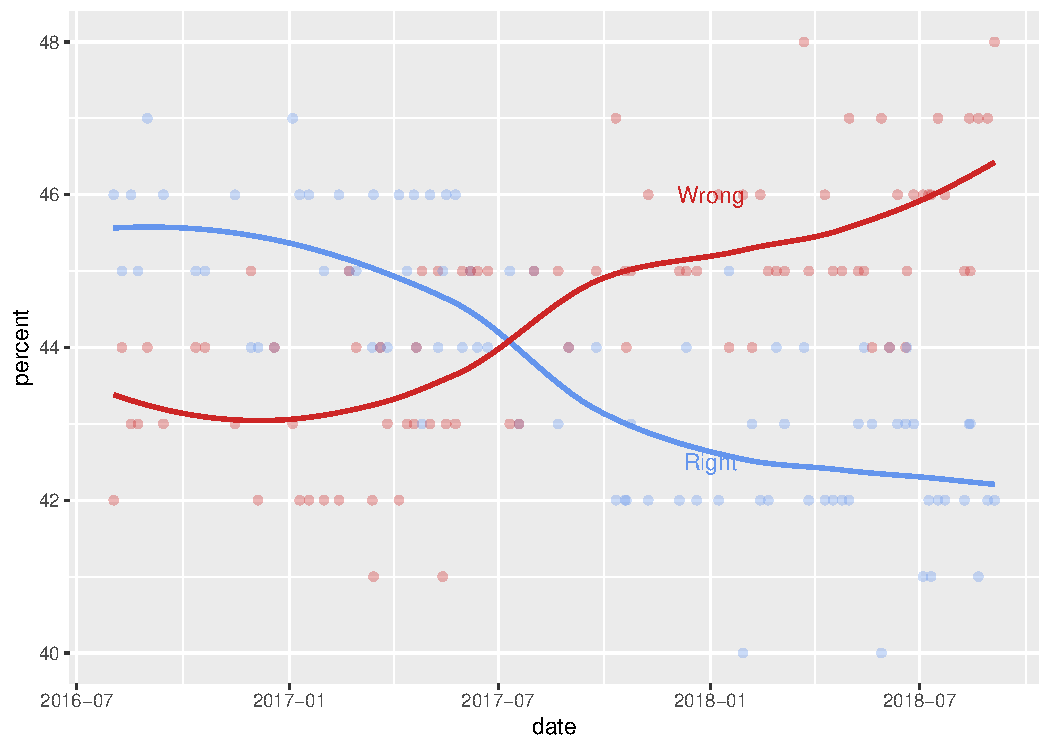
\includegraphics{03-intro-to-ggplot2_files/figure-latex/ggp_brexit_global_colors_text-1} \end{center}

These labels match up with the Medium article graph below:

\begin{center}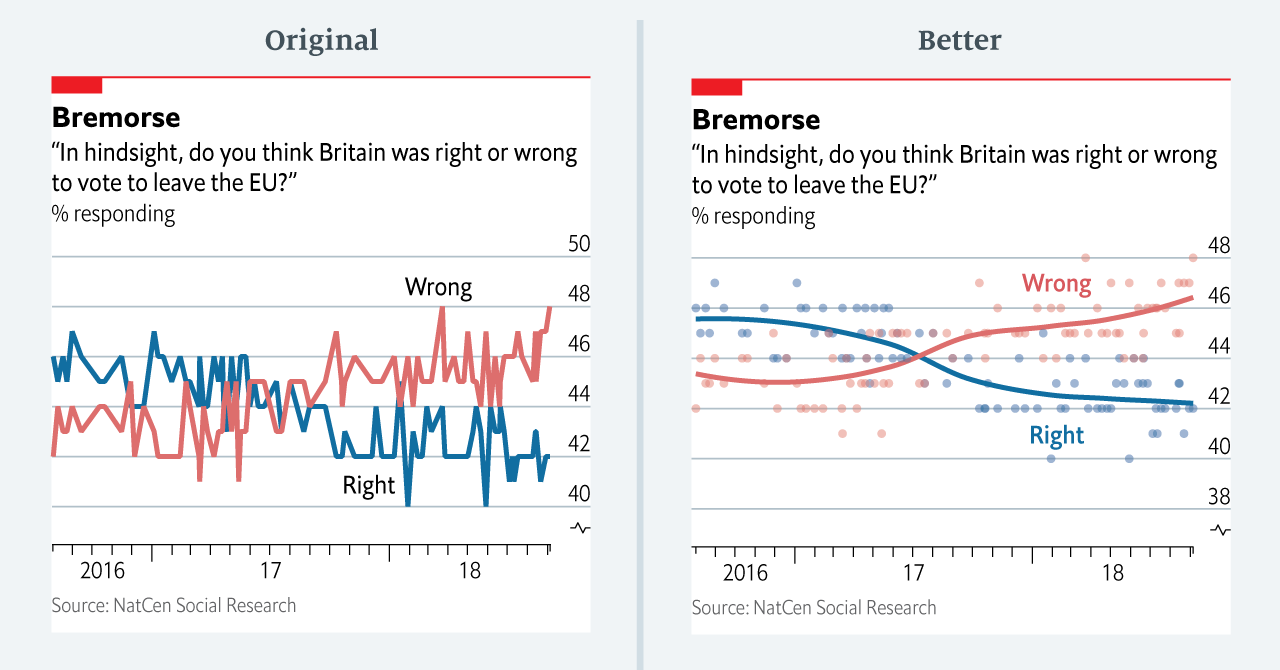
\includegraphics[width=7in,height=4in]{../img/original-brexit} \end{center}

In the next step, we will move the \texttt{y} axis over to the
right-hand side of the graph.

\hypertarget{adjusting-axes-on-a-graph}{%
\subsubsection{Adjusting axes on a
graph}\label{adjusting-axes-on-a-graph}}

Our graph is coming along, but we should shift the \texttt{y} axes to
the opposite side of the graph (like the image above).

\hypertarget{moving-the-y-axis}{%
\subsection{\texorpdfstring{\textbf{\emph{Moving the \texttt{y}
axis}}}{Moving the y axis}}\label{moving-the-y-axis}}

\texttt{ggplot2} has a rich grammar for building graphs, which means it
has a function for doing nearly anything we can think of, including
moving axes. To shift the \texttt{y} axis from it's original position,
we can use the \texttt{ggplot2::scale\_y\_continuous()} function and
specify \texttt{"right"} in the \texttt{position\ =} argument.

\begin{Shaded}
\begin{Highlighting}[]
\NormalTok{ggp\_brexit\_global\_colors\_text\_scale\_y }\OtherTok{\textless{}{-}}\NormalTok{ ggp\_brexit\_global\_colors\_text }\SpecialCharTok{+} 
\NormalTok{  ggplot2}\SpecialCharTok{::}\FunctionTok{scale\_y\_continuous}\NormalTok{(}\AttributeTok{position =} \StringTok{"right"}\NormalTok{)}
\NormalTok{ggp\_brexit\_global\_colors\_text\_scale\_y}
\end{Highlighting}
\end{Shaded}

\begin{center}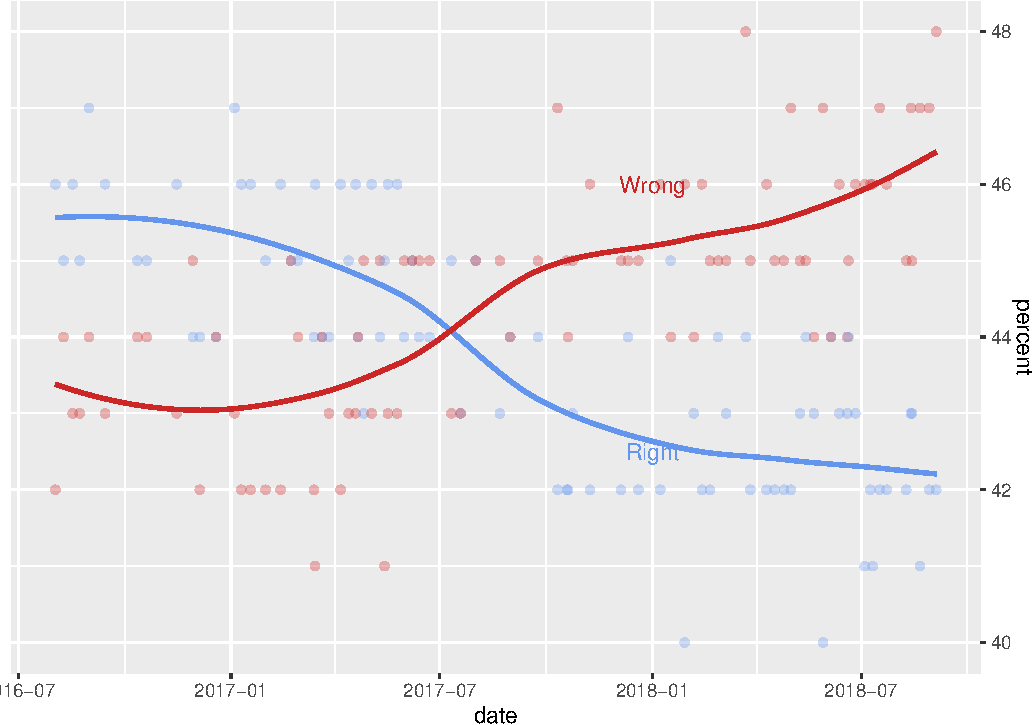
\includegraphics{03-intro-to-ggplot2_files/figure-latex/ggp_brexit_global_colors_text_scale_y-1} \end{center}

Now we have the lines, the points, the plot labels, and the axes in the
correct spot. Next up, we need to make sure our chart is titled and
labeled correctly!

\hypertarget{adding-labels}{%
\section{Adding labels}\label{adding-labels}}

Titles and labels are important because they give readers the context of
the information they see in a graph. Without some additional information
about the data, the audience is just staring at lines, points, colors,
etc.

\texttt{ggplot2} has a few options for labeling graphs, but we recommend
using the standard \texttt{ggplot2::labs()} function. It's easy to
remember, and it has most of the necessary arguments you'll need for
almost all the graphs you'll build.

\hypertarget{using-the-ggplot2labs-function}{%
\subsection{\texorpdfstring{\textbf{\emph{Using the
\texttt{ggplot2::labs()}
function}}}{Using the ggplot2::labs() function}}\label{using-the-ggplot2labs-function}}

Below is a set of arguments that match the title and labels from the
`Better' graph from the Medium article.

As you can see, the Economist article chose to remove the \texttt{x} and
\texttt{y} axes labels, but we think it's clearer to leave them in. Run
the code below to create the \texttt{labs\_eco} layer.

\begin{Shaded}
\begin{Highlighting}[]
\NormalTok{labs\_eco }\OtherTok{\textless{}{-}}\NormalTok{ ggplot2}\SpecialCharTok{::}\FunctionTok{labs}\NormalTok{(}\AttributeTok{title =} \StringTok{"Bremorse"}\NormalTok{, }
  \AttributeTok{subtitle =} \StringTok{"\textquotesingle{}In hindsight, do you think Britain was right or wrong to vote to leave the EU?\textquotesingle{}"}\NormalTok{, }
                \AttributeTok{caption =} \StringTok{"Source: NatCen Social Research"}\NormalTok{, }
                \AttributeTok{x =} \StringTok{" "}\NormalTok{, }
                \AttributeTok{y =} \StringTok{"Percent (\%)"}\NormalTok{)}
\end{Highlighting}
\end{Shaded}

We store the labels in the \texttt{labs\_eco} object, which we can add
to the \texttt{gg\_p13\_y} object and reassign this to the
\texttt{gg\_p14\_labs} object.

Run the code below to assign the labels layer to the plot object.

\begin{Shaded}
\begin{Highlighting}[]
\NormalTok{ggp\_brexit\_labs }\OtherTok{\textless{}{-}}\NormalTok{ ggp\_brexit\_global\_colors\_text\_scale\_y }\SpecialCharTok{+}\NormalTok{ labs\_eco}
\NormalTok{ggp\_brexit\_labs}
\end{Highlighting}
\end{Shaded}

\begin{center}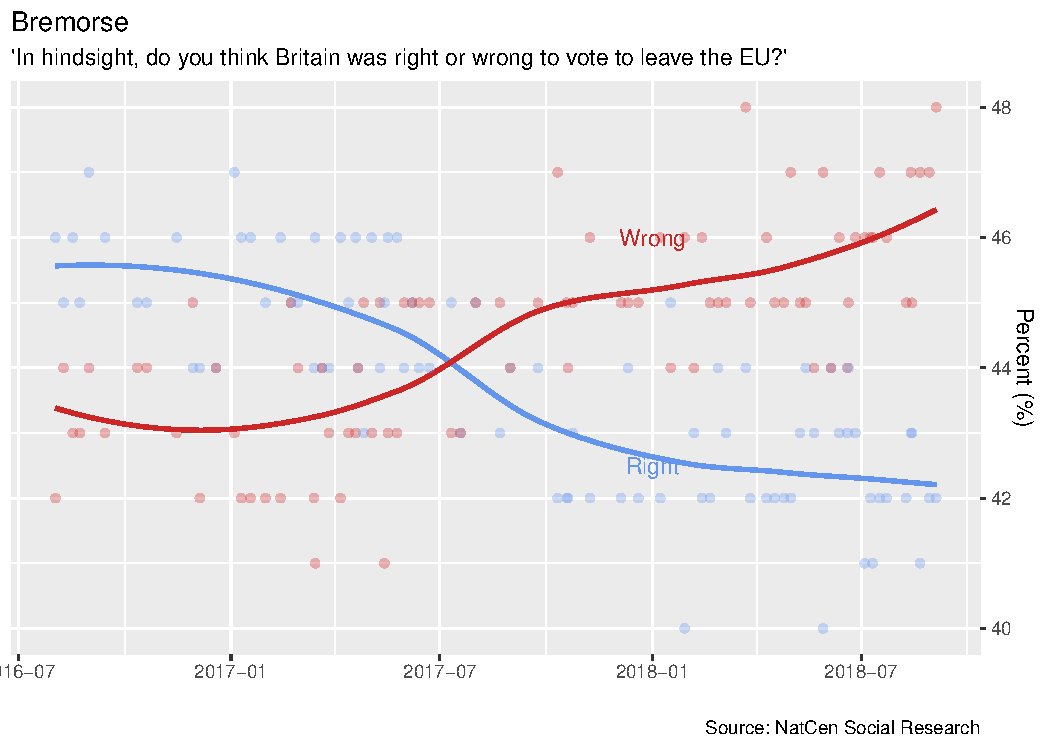
\includegraphics{03-intro-to-ggplot2_files/figure-latex/ggp_brexit_labs-1} \end{center}

Labels are also important for keeping track of your work. If you're
exploring a dataset using graphs (a process called
\href{https://en.wikipedia.org/wiki/Exploratory_data_analysis}{Exploratory
Data Analysis}, or EDA), the labels can help you remember what
transformations or changes you made to the data under hood.

\hypertarget{using-themes}{%
\section{Using themes}\label{using-themes}}

Our graph is nearly complete! We have all the geoms, aesthetics, titles,
and labels. The last thing we will add is a theme, but we will do this
by going outside the \texttt{tidyverse} to the
\href{https://yutannihilation.github.io/allYourFigureAreBelongToUs/ggthemes/}{\texttt{ggthemes}}
package.

\hypertarget{ggthemes}{%
\subsection{\texorpdfstring{\textbf{\emph{\texttt{ggthemes}}}}{ggthemes}}\label{ggthemes}}

The
\href{https://yutannihilation.github.io/allYourFigureAreBelongToUs/ggthemes/}{\texttt{ggthemes}
package} has pre-packaged design, color, and font choices for most
popular media outlets (FiveThirtyEight, Wall Street Journal, etc.).
We'll use the \texttt{ggthemes::theme\_economist\_white()} function to
change our plot's colors and design.

Install this package by clicking on the code section below:

\begin{Shaded}
\begin{Highlighting}[]
\FunctionTok{install.packages}\NormalTok{(}\StringTok{"ggthemes"}\NormalTok{)}
\FunctionTok{library}\NormalTok{(ggthemes)}
\end{Highlighting}
\end{Shaded}

This function takes a \texttt{gray\_bg\ =} argument, which we will set
to \texttt{FALSE}. We'll also change the \texttt{base\_size} for the
font to \texttt{12}, and the default font family to \texttt{"Verdana"}.

\begin{Shaded}
\begin{Highlighting}[]
\NormalTok{ggp\_brexit\_labs }\SpecialCharTok{+} 
\NormalTok{  ggthemes}\SpecialCharTok{::}\FunctionTok{theme\_economist\_white}\NormalTok{(}\AttributeTok{gray\_bg =} \ConstantTok{FALSE}\NormalTok{, }
                                 \AttributeTok{base\_size =} \DecValTok{12}\NormalTok{, }
                                 \AttributeTok{base\_family =} \StringTok{"Verdana"}\NormalTok{)}
\end{Highlighting}
\end{Shaded}

\begin{center}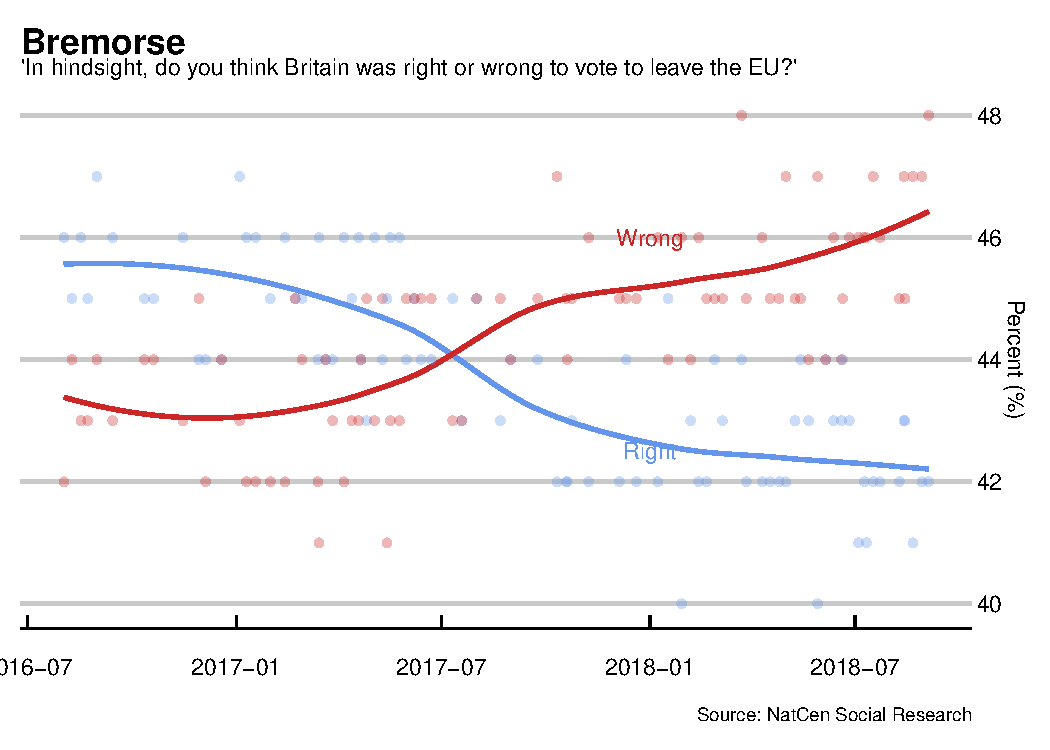
\includegraphics{03-intro-to-ggplot2_files/figure-latex/theme_economist_white-1} \end{center}

This looks pretty close, right? Compare to the image below:

\begin{center}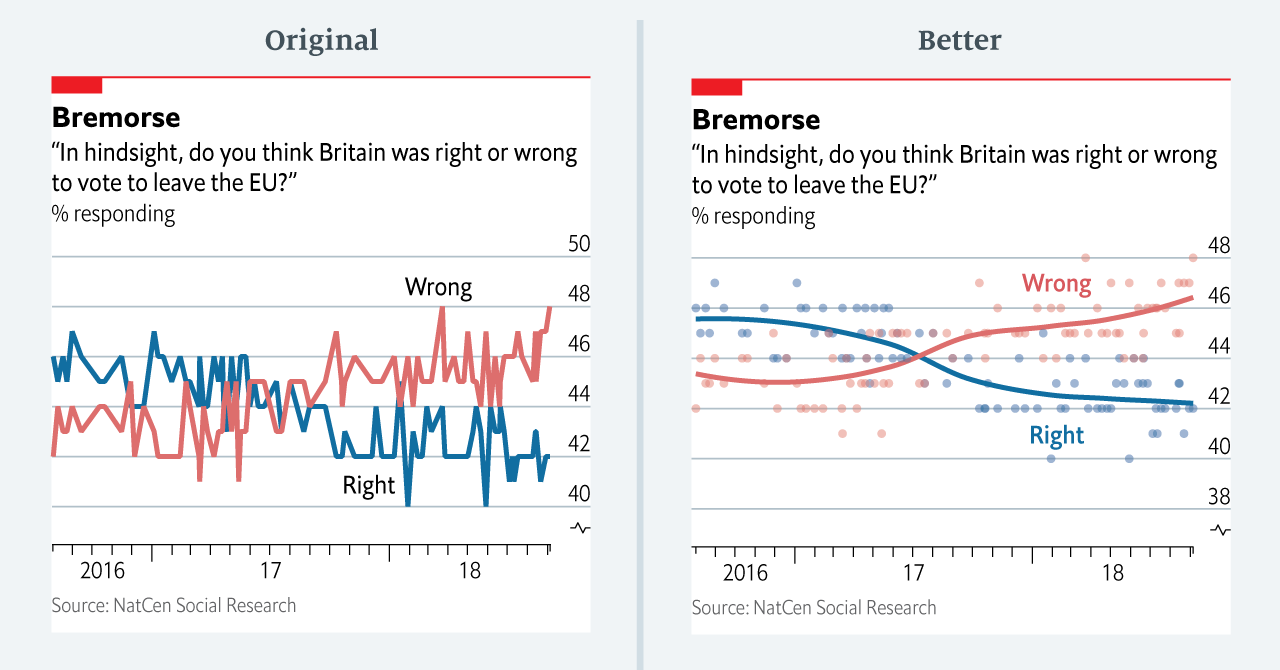
\includegraphics[width=7in,height=4in]{../img/original-brexit} \end{center}

%\showmatmethods





\end{document}
